% This is the HU Berlin LaTeX template, optimized for R Markdown.

% -------------------------------
% --- PREAMBLE ---
% -------------------------------
\documentclass[a4paper,11pt]{article}
\usepackage[T1]{fontenc}
\usepackage[utf8]{inputenc}
\usepackage{tgtermes}
\usepackage{amsmath,amssymb,amsfonts,amsthm}    % Typical maths resource packages
\usepackage{graphicx}                           % Packages to allow inclusion of graphics
\usepackage[bf]{caption}
\usepackage{textcomp}                           % For single quotes
\usepackage{floatrow}                           % For image and table position
\usepackage{booktabs}                           % For tables
%\usepackage[driverfallback=hypertex]{hyperref}                          
% \usepackage[bottom]{footmisc}                   
\usepackage[bottom, flushmargin]{footmisc}                   % For footnotes
\usepackage[citebordercolor={0 1 0}]{hyperref}               % For creating hyperlinks in cross references
\usepackage{footnotebackref}
\usepackage{setspace}
\usepackage{float}
\usepackage{ragged2e}
\usepackage{tabularx}

% -------------------------------
% --- some layout definitions ---
% -------------------------------

% define topline
\usepackage[automark]{scrlayer-scrpage}
\pagestyle{scrheadings}
\automark{section}
\clearscrheadings
\ohead{\headmark}




% define page size, margin size
\setlength{\headheight}{1.1\baselineskip}
\voffset=-2cm
\hoffset=-3cm
\textheight24cm
\textwidth15.5cm
\topmargin1cm
\oddsidemargin3cm
\evensidemargin3cm
\setcounter{secnumdepth}{3}
\setcounter{tocdepth}{3}   
  \usepackage[parfill]{parskip} 

% define line spacing = 1.5
\renewcommand{\baselinestretch}{1.5}

% define position of graphics
\floatsetup[figure]{capposition=bottom}
\floatsetup[table]{capposition=bottom}
\floatplacement{figure}{ht}
\floatplacement{table}{ht}

% save thesis parameters for later
\newcommand{\thesistype}{Master's Thesis}
\newcommand{\thesisauthor}{Elias Cuadra Braatz}
\newcommand{\thesisdate}{August 04, 2021}

% define tightlist to work with newer versions of pandoc
\providecommand{\tightlist}{%
  \setlength{\itemsep}{0pt}\setlength{\parskip}{0pt}}

% change spacing
\setlength {\parskip}{1em}

% Additional LaTeX parameters added in the YAML header of index.Rmd


%fix csl issue
\newlength{\cslhangindent}
\setlength{\cslhangindent}{1.5em}
\newlength{\csllabelwidth}
\setlength{\csllabelwidth}{3em}
\newenvironment{CSLReferences}[3] % #1 hanging-ident, #2 entry spacing
 {% don't indent paragraphs
  \setlength{\parindent}{0pt}
  % turn on hanging indent if param 1 is 1
  \ifodd #1 \everypar{\setlength{\hangindent}{\cslhangindent}}\ignorespaces\fi
  % set entry spacing
  \ifnum #2 > 0
  \setlength{\parskip}{#2\baselineskip}
  \fi
 }%
 {}
\usepackage{calc} % for \widthof, \maxof
\newcommand{\CSLBlock}[1]{#1\hfill\break}
\newcommand{\CSLLeftMargin}[1]{\parbox[t]{\maxof{\widthof{#1}}{\csllabelwidth}}{#1}}
\newcommand{\CSLRightInline}[1]{\parbox[t]{\linewidth}{#1}}
\newcommand{\CSLIndent}[1]{\hspace{\cslhangindent}#1}

%fix code issue
\usepackage{color}
\usepackage{fancyvrb}
\newcommand{\VerbBar}{|}
\newcommand{\VERB}{\Verb[commandchars=\\\{\}]}
\DefineVerbatimEnvironment{Highlighting}{Verbatim}{commandchars=\\\{\}}
% Add ',fontsize=\small' for more characters per line
\usepackage{framed}
\definecolor{shadecolor}{RGB}{248,248,248}
\newenvironment{Shaded}{\begin{snugshade}}{\end{snugshade}}
\newcommand{\AlertTok}[1]{\textcolor[rgb]{0.94,0.16,0.16}{#1}}
\newcommand{\AnnotationTok}[1]{\textcolor[rgb]{0.56,0.35,0.01}{\textbf{\textit{#1}}}}
\newcommand{\AttributeTok}[1]{\textcolor[rgb]{0.77,0.63,0.00}{#1}}
\newcommand{\BaseNTok}[1]{\textcolor[rgb]{0.00,0.00,0.81}{#1}}
\newcommand{\BuiltInTok}[1]{#1}
\newcommand{\CharTok}[1]{\textcolor[rgb]{0.31,0.60,0.02}{#1}}
\newcommand{\CommentTok}[1]{\textcolor[rgb]{0.56,0.35,0.01}{\textit{#1}}}
\newcommand{\CommentVarTok}[1]{\textcolor[rgb]{0.56,0.35,0.01}{\textbf{\textit{#1}}}}
\newcommand{\ConstantTok}[1]{\textcolor[rgb]{0.00,0.00,0.00}{#1}}
\newcommand{\ControlFlowTok}[1]{\textcolor[rgb]{0.13,0.29,0.53}{\textbf{#1}}}
\newcommand{\DataTypeTok}[1]{\textcolor[rgb]{0.13,0.29,0.53}{#1}}
\newcommand{\DecValTok}[1]{\textcolor[rgb]{0.00,0.00,0.81}{#1}}
\newcommand{\DocumentationTok}[1]{\textcolor[rgb]{0.56,0.35,0.01}{\textbf{\textit{#1}}}}
\newcommand{\ErrorTok}[1]{\textcolor[rgb]{0.64,0.00,0.00}{\textbf{#1}}}
\newcommand{\ExtensionTok}[1]{#1}
\newcommand{\FloatTok}[1]{\textcolor[rgb]{0.00,0.00,0.81}{#1}}
\newcommand{\FunctionTok}[1]{\textcolor[rgb]{0.00,0.00,0.00}{#1}}
\newcommand{\ImportTok}[1]{#1}
\newcommand{\InformationTok}[1]{\textcolor[rgb]{0.56,0.35,0.01}{\textbf{\textit{#1}}}}
\newcommand{\KeywordTok}[1]{\textcolor[rgb]{0.13,0.29,0.53}{\textbf{#1}}}
\newcommand{\NormalTok}[1]{#1}
\newcommand{\OperatorTok}[1]{\textcolor[rgb]{0.81,0.36,0.00}{\textbf{#1}}}
\newcommand{\OtherTok}[1]{\textcolor[rgb]{0.56,0.35,0.01}{#1}}
\newcommand{\PreprocessorTok}[1]{\textcolor[rgb]{0.56,0.35,0.01}{\textit{#1}}}
\newcommand{\RegionMarkerTok}[1]{#1}
\newcommand{\SpecialCharTok}[1]{\textcolor[rgb]{0.00,0.00,0.00}{#1}}
\newcommand{\SpecialStringTok}[1]{\textcolor[rgb]{0.31,0.60,0.02}{#1}}
\newcommand{\StringTok}[1]{\textcolor[rgb]{0.31,0.60,0.02}{#1}}
\newcommand{\VariableTok}[1]{\textcolor[rgb]{0.00,0.00,0.00}{#1}}
\newcommand{\VerbatimStringTok}[1]{\textcolor[rgb]{0.31,0.60,0.02}{#1}}
\newcommand{\WarningTok}[1]{\textcolor[rgb]{0.56,0.35,0.01}{\textbf{\textit{#1}}}}




% --------------------------------------
% --------------------------------------
% --------------------------------------
% --- the structure the tex document ---
% ---  (this our recommendation) -------
% frontmatter:
%   - titlepage (mandatory),
%   - acknowledgement,
%   - abstract,
%   - table of contents (mandatory),
%   - list of abbreviations (not mandatory),
%   - list of figures (not mandatory),
%   - list of tables  (not mandatory) .
%
% body of the thesis (the structure of the thesis body is not mandatory, but the list of literature is mandatory):
%   - introduction,
%   - methods,
%   - data,
%   - results,
%   - conclusion,
%   - literature (mandatory),
%   - appendix (figures, tables).
%
% last page:
%   - declaration of authorship (mandatory).
% --------------------------------------
% --------------------------------------
% --------------------------------------
\begin{document}

% -------------------------------
% --- frontmatter: Title page ---
% -------------------------------
\thispagestyle{empty}
\begin{center}
  \vspace*{5mm}
  \linespread{1.5}
  {\huge{\bf Windenergy and Repowering potential in Rhineland-Palatinate from 2021 to 2030}\par}\vspace{1cm}
  Master's Thesis submitted \\\vspace{0.5cm}
  to \\\vspace{0.5cm}
  \textbf{Dr.~Stefan Jergentz} \\
  \textbf{Dr.~Nanki Sidhu} \\\vspace{1.5cm}
  
  
  \includegraphics[width=0.5\textwidth]{Uni-Logo-2.jpg}
  
  Institute of Environmental Sciences \\
  Environmental Economics \\
   Chair: Prof.~Oliver Frör \\  \vspace{1cm}

  
  
  by \\\vspace{0.5cm}
  \textbf{Elias Cuadra Braatz} \\
  (219202265) \\
  
  \medskip
  \medskip
  in partial fulfillment of the requirements \\
  for the degree of \\
  \textbf{Master of Environmental Sciences} \\\vspace{0.5cm}
  August 04, 2021
  
\end{center}


% -----------------------------
% --- frontmatter: Contents ---
% -----------------------------
\newpage
\tableofcontents
\clearpage

% -----------------------------
% --- frontmatter: Abstract ---
% -----------------------------
\newpage
\hypertarget{abstract}{%
\section*{Abstract}\label{abstract}}
\addcontentsline{toc}{section}{Abstract}

This is the template for a thesis at the Chair of Econometrics of
Humboldt--Universit"at zu Berlin. A popular approach to write a thesis or a
paper is the IMRAD method (Introduction, Methods, Results and Discussion). This
approach is not mandatory! You can find more information about formal
requirements in the booklet `Hinweise zur Gestaltung der äußeren Form von
Diplomarbeiten' which is available in the office of studies.

The abstract should not be longer than a paragraph of around 10-15 lines (or
about 150 words). The abstract should contain a concise description of the
econometric/economic problem you analyze and of your results. This allows the
busy reader to obtain quickly a clear idea of the thesis content.

% ----------------------------------------------------------
% --- frontmatter: List of Abbreviations (not mandatory) ---
% ----------------------------------------------------------
\newpage
\hypertarget{list-of-abbreviations}{%
\section*{List of Abbreviations}\label{list-of-abbreviations}}
\addcontentsline{toc}{section}{List of Abbreviations}
\begin{tabular}{rp{0.2cm}lp{1cm}rp{0.2cm}l}
    CPI     & &  Consumer Price Index   & & ETF     & &  Equity Traded Funds  \\
    ETH     & &  Eat the Horse          & & XLM     & &  Xetra Liquidity
\end{tabular}
% ----------------------------------------------------
% --- frontmatter: List of Figures (not mandatory) ---
% ----------------------------------------------------
\newpage
\listoffigures
\addcontentsline{toc}{section}{List of Figures}

% ---------------------------------------------------
% --- frontmatter: List of Tables (not mandatory) ---
% ---------------------------------------------------
\newpage
\listoftables
\addcontentsline{toc}{section}{List of Tables}

% -------------------------------
% --- main body of the thesis ---
% -------------------------------
\newpage
\pagestyle{plain}       
\setcounter{page}{1}    % start page numbering anew
\pagenumbering{arabic}  % page numbers in arabic style

\hypertarget{introduction}{%
\section{Introduction}\label{introduction}}

This work was executed and written in scientific recognition of the importance of reducing greenhouse gas emissions and expanding renewable energies to mitigate the effects of climate change.

This study was also carried out on behalf of the state-owned energy agency {[}\protect\hyperlink{ref-EnergieagenturRheinlandPfalz.2021}{1}{]} within the project ``municipal greenhouse gas accounting and regional climate protection portals in Rhineland-Palatinate'' {[}\protect\hyperlink{ref-KomBiReK.2021}{2}{]}, which is funded by the ``European Regional Development Fund'' {[}\protect\hyperlink{ref-EuropeanRegionalDevelopmentFund.2021}{3}{]} and the state of Rhineland-Palatinate (RLP). This project supports the creation of municipal climate protection measures in order to achieve the climate protection goals of the municipalities and the state and thereby increases regional added value, ensures sustainability and thus improves the quality of life of all citizens. When developing municipal climate protection, a sound strategy is required regarding the legally anchored striving for climate neutrality of the state of RLP {[}\protect\hyperlink{ref-RheinlandPfalz.19.08.2014}{4}{]}. Even more pressure comes from the recent press release No.~31/2021 of April 29 in 2021 {[}\protect\hyperlink{ref-Bundesverfassungsgericht.24.03.2021}{5}{]}, in which the first Senate of the Federal Constitutional Court decided that the regulations of the Climate Protection Act of December 12 in 2019 {[}\protect\hyperlink{ref-BundesamtfurJustiz.2019}{6}{]} on the national climate protection targets and the annual emission quantities permitted up to 2030 are incompatible with fundamental rights, as there are no sufficient criteria for further emission reductions from 2031 onward. It is stated that the legal requirements are not sufficient to bring about a timely transition to climate neutrality. The German legislature has therefore published an adjusted edition of this act that strives for a faster development of renewable energies and the energy transition in general {[}\protect\hyperlink{ref-BundesministeriumfurUmweltNaturschutzundnukleareSicherheit.12.05.2021}{7}{]}. This shows that this study is highly embedded in a socio-economic context. The energy transition is a cornerstone of a decent strategy to climate neutrality and RLP wants to play a pioneering role in the implementation of the energy transition. The state government publishes on its website that RLP will cover 100 \% of its electricity needs from renewable energies by 2030 {[}\protect\hyperlink{ref-LandesregierungRheinlandPfalz.2021}{8}{]}. In addition to energy from the sun, water and biomass, two thirds of the electricity generated in 2030 should come from wind power and is therefore the subject of this master thesis. The study area and the modeled wind speeds taken from the Windatlas RLP {[}\protect\hyperlink{ref-MinisteriumfurWirtschaftKlimaschutzEnergieundLandesplanung.2013}{9}{]} are seen in figure \ref{fig:wind}.

The gross electricity generation in RLP from wind power rose in 2017 with 5.9 TWh to 29 \% of the total 20.7 TWh generated electricity. The total consumption in the same year was 29.1 TWh {[}\protect\hyperlink{ref-Lehnert.2020}{10}{]}. In the year 2019 the electricity generation from WT's was already 6.7 TWh. It can be assumed that, on the one hand, electricity consumption will increase in the future due to the electrification of transport and domestic heating, and on the other hand, efficiency measures can also lead to a lower energy consumption. Whereas some past studies and scenarios estimated a slight increase and some a slight decrease but on average a relatively unchanged electricity consumption in Germany {[}\protect\hyperlink{ref-NormanGerhardt.2015}{11}{]}, the newest press release of the Federal Ministry for Economic Affairs and Energy makes is clear that an increase of about 12 \% is expected {[}\protect\hyperlink{ref-AndreasMertens.13.07.2021}{12}{]}. and further studies will follow in the autumn of 2021. In order to achieve the self-set goals of using two thirds of the electricity demand from wind power with an estimated electricity demand of 33 TWh in 2030 in RLP, electricity supply from with wind turbines (WT's) must be about 22 TWh per year if RLP wants to become independent of electricity imports. There are two ways of increasing the amount of electricity generated by wind energy. On the one hand, areas that are still available can be identified and built on with new WT's. On the other hand, existing old systems, whose absolute electricity feed-in quantity is low, can be replaced by new, higher and more efficient systems through the so-called ``repowering.''
The aim of this work is to develop a methodology for calculating the wind energy potential and its related area consumption at the state level as well as for the districts and association communities in RLP. With this results an evaluation of the desired expansion targets should be assessed. The central three questions of this work are therefore:
\begin{enumerate}
\def\labelenumi{\arabic{enumi}.}
\item
  How much electric energy can be generated by a new wind turbine from 2021 until 2030 in RLP per area?
\item
  How large is the potential when all wind turbines with a commissioning date before 2005 are repowered?
\item
  How much area is needed to generate the target amount of 22 TWh out of wind energy?
\end{enumerate}
In order to answer these questions, the technical fundamentals of the electricity yield from WT's are explained first. Subsequently, the master and movement data provided by the transmission system operator Amprion, which contains all electricity fed into the public grid by WT's and other technical information, is analyzed and forecasted up to the year 2030. The respective area consumption to generate that electricity is calculated using a GIS based approach and data from the market master data register (Marktstammdatenregister - MaStR). As a by-product the greenhouse gas reduction potential can be derived from the potential for electricity generation. Knowing the electricity potential per area, the required area for the generation targets can be calculated and an assessment of the given expectations can be made subsequently.


\begin{figure}[H]

{\centering 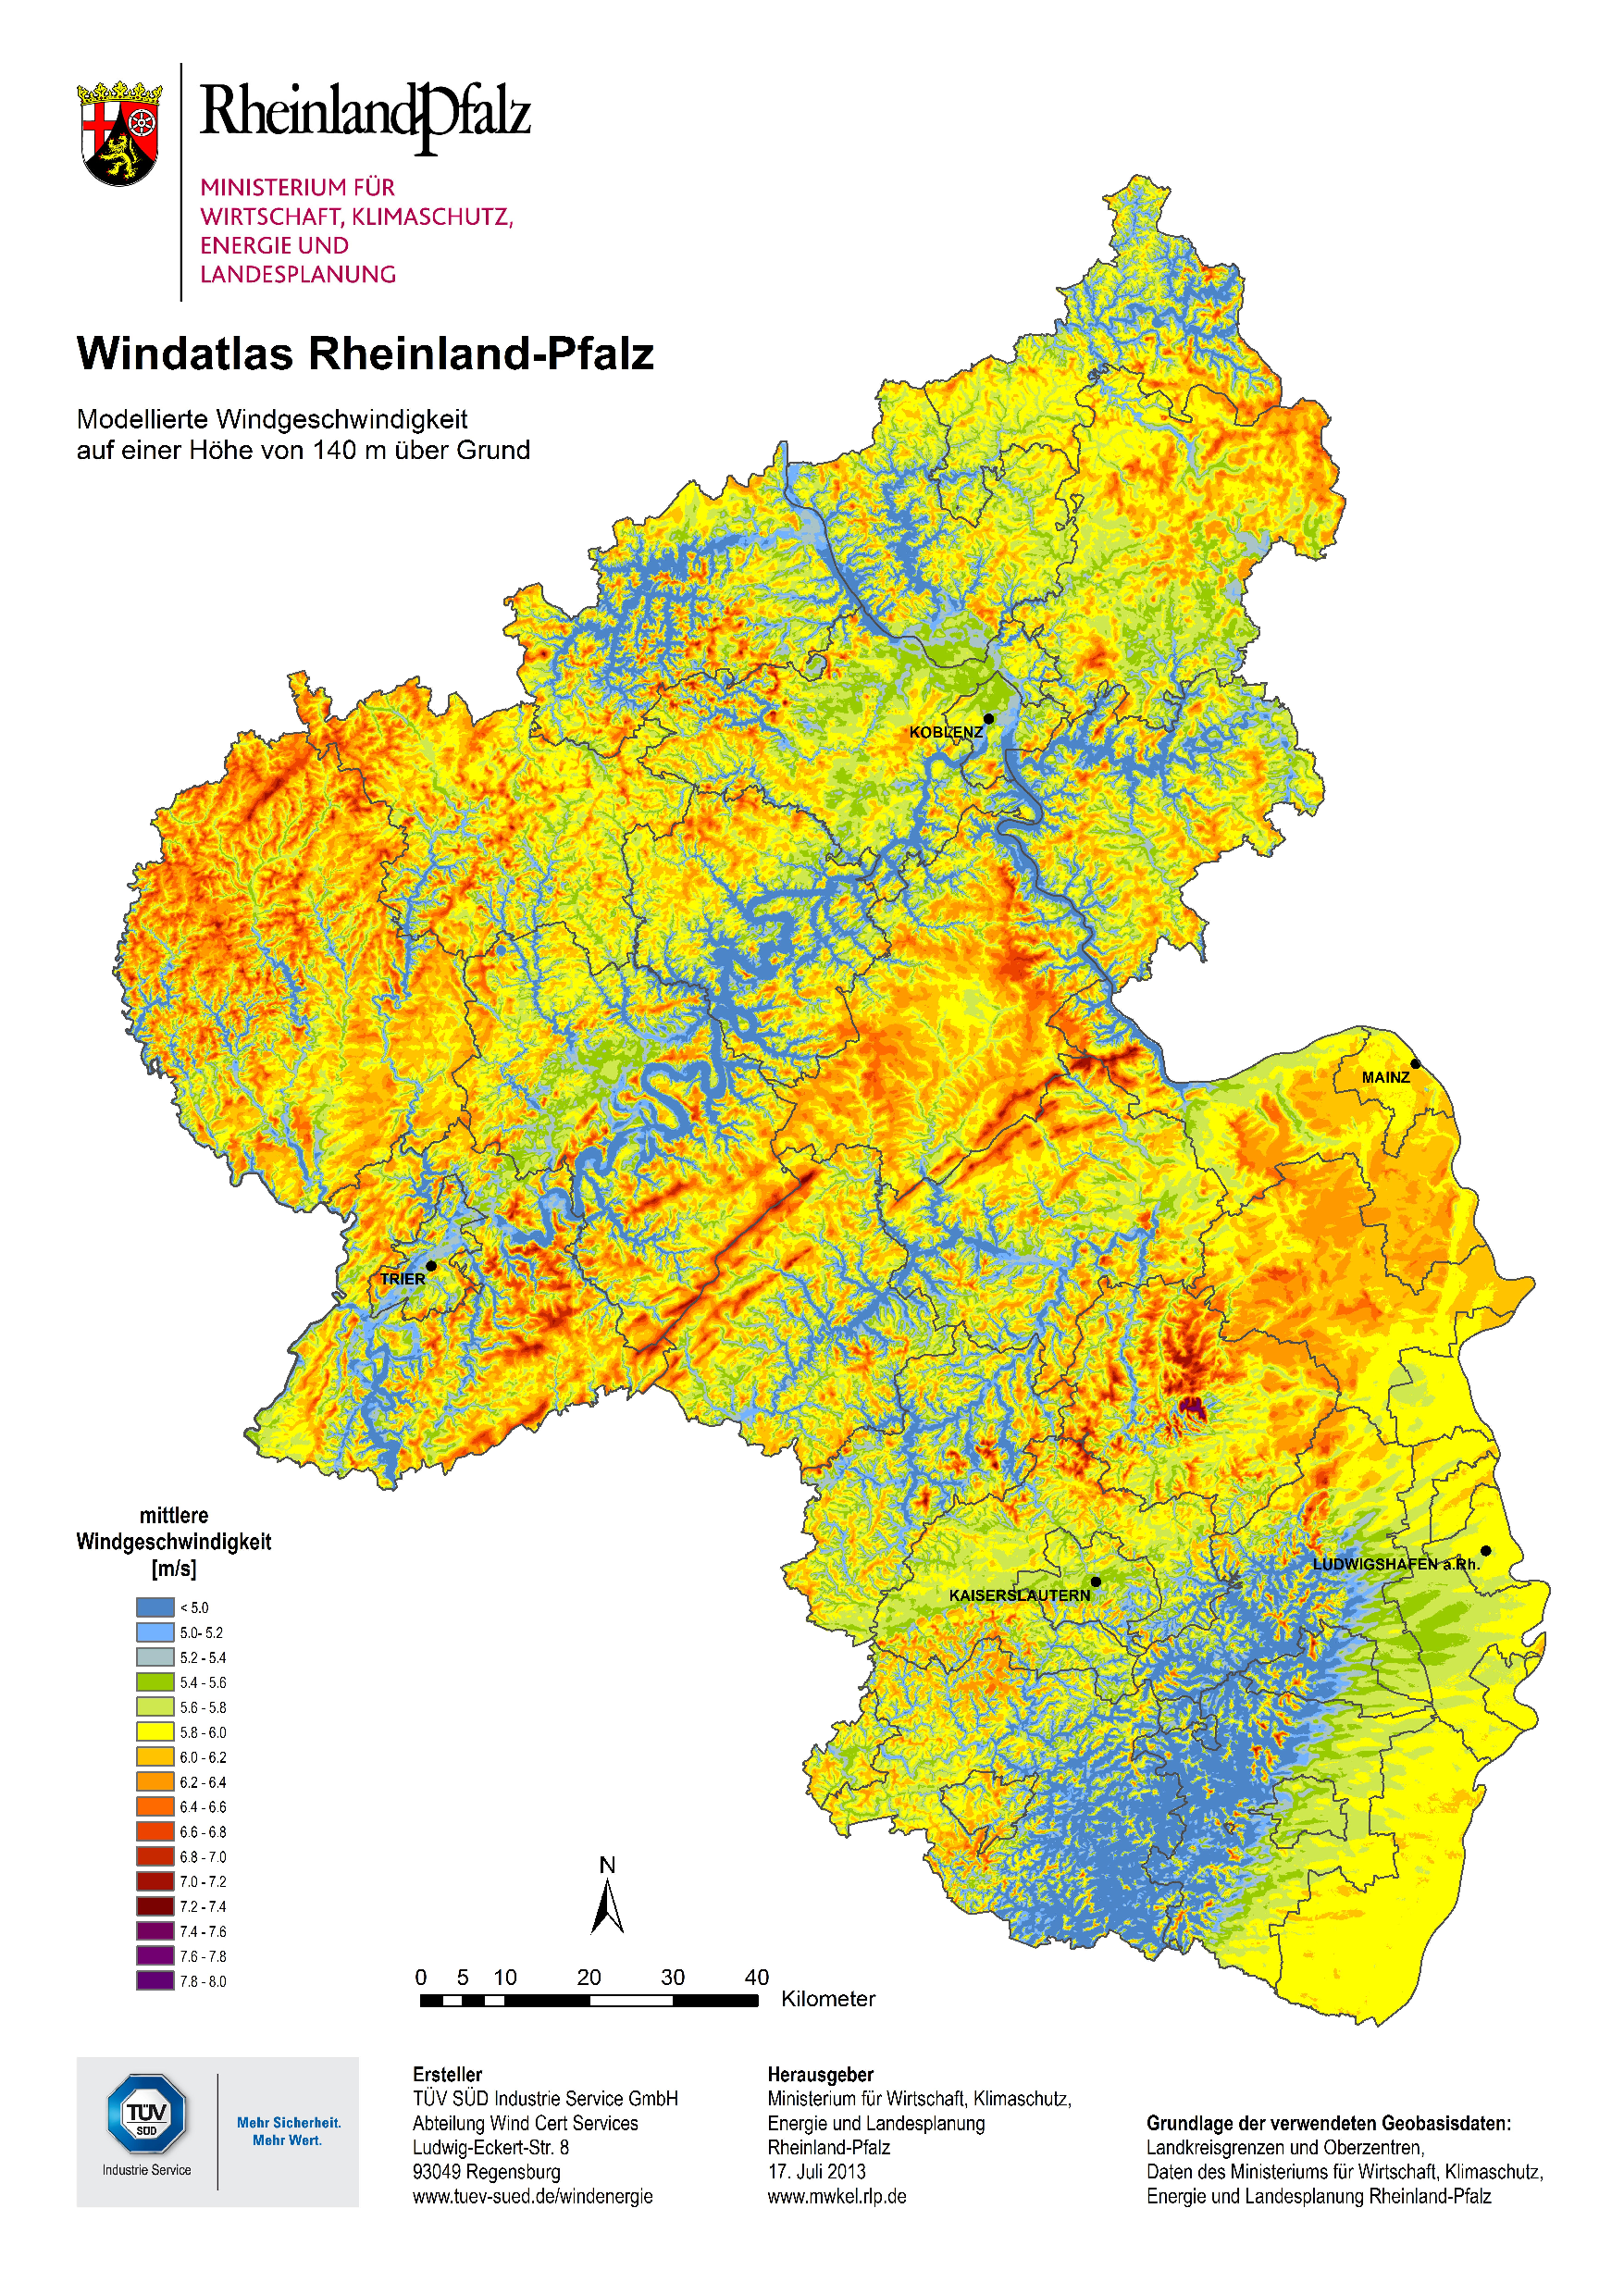
\includegraphics[width=1\linewidth]{figures/wind_140m} 

}

\caption{Wind speeds in RLP 140 m above Ground {[}\protect\hyperlink{ref-MinisteriumfurWirtschaftKlimaschutzEnergieundLandesplanung.2013}{9}{]}.}\label{fig:wind}
\end{figure}
\hypertarget{state-of-the-art}{%
\section{State of the art}\label{state-of-the-art}}

\hypertarget{physical-basics}{%
\subsection{Physical basics}\label{physical-basics}}

Wind energy has been used by humans for thousands of years, but the generation of electrical power has only been possible since the 19th century with the beginning of industrialization and is now the subject of constant research and development in the context of the energy transition {[}\protect\hyperlink{ref-Wikipedia.2021}{13}{]}. A wind turbine usually consists of the three main components; rotor blades, nacelle and tower. Besides other elements the nacelle contains; the gearbox, the generator, the transformer and the control system {[}\protect\hyperlink{ref-MladenBosnjakovic.2013}{14}{]}. The mostly three rotor blades are attached to the rotor hub and absorb the kinetic energy of the wind and convert it into a rotary motion. If the winds are too strong, the rotor blades can be ``taken out of the wind'' by adjusting the blades, thus protecting the system from damage. Mainly the gearbox and the generator convert the kinetic energy into electricity. However, there are also systems with direct drive and without gear. The nacelle can be rotated to an optimal position when the wind conditions change, and an electromagnetic brake helps to shut down the system when the winds are too strong or during maintenance work. In addition to its load-bearing function, the tower also contains the power lines that conduct electricity to the grid connection of the distribution network {[}\protect\hyperlink{ref-NetzKonstrukteur.16.11.2020}{15}{]}.

The transmission system operators, in this case Amprion, are obliged to publish so-called master and movement data for each calendar year in accordance with section 77 Renewable Energy Act 2017 {[}\protect\hyperlink{ref-Bundesgestzblatt.2017}{16}{]}. These movement data include the annual electricity generation and the system key. The movement data for RLP are currently available until 2019. The total amount of electricity fed in with remuneration in 2019 from wind turbines in RLP is 6,782,180,753 kWh, i.e.~approx. 6.782 TWh {[}\protect\hyperlink{ref-EnergieagenturRheinlandPfalz.2019}{17}{]}.

The amount of electricity generated by a wind turbine, the electricity yield, can be derived from the physical relationship between the kinetic energy and the power of the wind. Without claiming to be exhaustive, the following applies\footnote{\(E_{kin}= kinetic\; energy,\; m=mass\; of\; air,\; v= wind\;speed\)}:
\begin{equation}
E_{kin} = \frac{1}{2}mv^2
\end{equation}
The air throughput or mass flow \(\hat{m}\) that flows through the area swept by the rotor blades can be calculated by multiplying the air density, rotor area and wind speed as well as the time interval required with\footnote{\(\rho= density\; of\; air,\; A= rotor\; area\)}:
\begin{equation}
\hat{m}=\rho A vt
\end{equation}
The power P is equal to the energy per unit of time \(\hat{E}\). This results in the power of the wind with\footnote{\(r= radius\; of\; rotor\)}:
\begin{equation}
P_{wind}=\hat{E}=\frac{1}{2}\hat{m}v^2=\frac{1}{2} \rho \pi r^2 v^3
\end{equation}
(Mac Kay {[}\protect\hyperlink{ref-DavidJCMacKay.2009}{18}{]} and BWE {[}\protect\hyperlink{ref-BWE.2021}{19}{]})

In Formula 3 it becomes clear that the wind speed is the decisive factor for the performance of a WT. Because WT's are build to perform at lower wind speeds most of the time they can not operate at very high wind speeds an have to be taken out of the wind at a certain speed to avoid fatigue and destruction through peak loads. A typical load profile of a WT is shown in figure \ref{fig:powerofwind}. If the density of air is 1.3 kg per m³ and there is an average windspeed of 6 m/s, which could be realistic for many sites in RLP in 140 m above ground, as seen in figure \ref{fig:wind}, then the typical power of the wind per square meter hoop is:
\begin{equation}
\begin{split}
\frac{1}{2} \rho v^3=\frac{1}{2}1.3 kg/m^3 * (6 m/s)^3=140 W/m^2 \\
with 1 \frac{kg m^2}{s^3} = 1 W
\end{split}
\end{equation}
The curve of power per m\textsuperscript{2} in relation to the wind speed is also shown in figure \ref{fig:powerofwind}.
\begin{figure}

{\centering \includegraphics[width=0.49\linewidth,height=0.25\textheight]{figures/power2} \includegraphics[width=0.49\linewidth,height=0.25\textheight]{figures/Typical-wind-power-output-versus-wind-speed_W640} 

}

\caption{Left: Power of the wind per area over wind speed; Right: Typical load profile of a WT}\label{fig:powerofwind}
\end{figure}
Of course, not all the wind's power can be converted and there are further losses when converting kinetic energy into electrical energy in the generator. The efficiency using the winds energy in theory after Alber Betz is a maximum of 59 \% also called the Betz limit {[}\protect\hyperlink{ref-A.Betz.1920}{20}{]}, but in practice it is often around 40 \% to a maximum of 50 \% {[}\protect\hyperlink{ref-WindwartsEnergieausdemNorden.2021}{21}{]}. If the average rotor diameter installed in RLP in 2020 was 130 m (figure \ref{fig:rotor}) with an efficiency of 50 \%, then the average power of one WT is:
\begin{equation}
\begin{split}
P_{WT} & = 0.5 * \frac{1}{2} \rho v^3 * \frac{\pi}{4}d^2 \\
P_{WT130} & = 70 W/m^2 * \frac{\pi}{4}(130 m)^2 = 929 kW
\end{split}
\end{equation}
The amount of energy also increases proportionally with increasing rotor diameter. This explains why the rotor diameters become larger in practice (figure \ref{fig:rotor}). But WT's with larger rotors have to be spaced further appart. In the literature values from 3 to 8 times the rotor diameter depending on the main direction of the wind can be found {[}\protect\hyperlink{ref-DavidJCMacKay.2009}{18}{]}. If we assume further that windmills in RLP are spaced on average 5 times their diameter apart from each other, from equation 5 follows that the energy per area land mass is:
\begin{equation}
\begin{split}
\frac{P_{WT}}{m^2} & = \frac{\frac{1}{2} \rho v^3 \frac{\pi}{8}d^2}{(5d)^2} \\
 & = \frac{\pi}{200} \frac{1}{2} \rho v^3 \\
 & = 0.016 * 140 W/m^2 \\
 & = 2.2 W/m^2
\end{split}
\end{equation}
This means that independently of the rotor size, there is a limit of around 2.2 W/m\textsuperscript{2} of electrical energy that can be delivered in Rhineland-Palatinate assuming an average wind speed of about 6 m/s. In the literature values for the electric power per area vary from 1 to 7 W/m\textsuperscript{2} land mass depending on the site conditions {[}\protect\hyperlink{ref-SvenLinow.2020}{22}{]}. Nonetheless, building higher WT's can be beneficial due to higher and more constant wind speeds with increasing height and other economic factors. As a rough estimate it can be said that doubling the height increases wind-speed by 10 \% and thus increase the power of the wind by 30 \% and therefore the hub heights also tend to increase (figure \ref{fig:nabe}). The actual way that wind speed increases with heigth is much more complicated and depends on the roughness of the surrounding area and time and is beyond of the scope of this study. Usually WT's are design to start operating at wind speeds around 3 to 5 m/s and stop at around 25 m/s. A WT has a so-called ``capacity'' or ``peak power'' which is the maximum power that the WT can generate in optimal conditions. The actual average power that is delivered can be expressed by the capacity multiplied by a factor that describes the fraction of the time that wind conditions are near optimal. This factor can be called the ``load factor'' and a typical load factor in Germany is around 19 \%, 22 \% in the Netherlands and 30 \% in the United Kingdom {[}\protect\hyperlink{ref-DavidJCMacKay.2009}{18}{]}. Lastly it can be estimated how much area is needed when we assume a rounded and constant electricity yield of 2 W/m\textsuperscript{2} and an electricity demand of 20 TWh per year in RLP:
\begin{equation}
A_{20TWh}=\frac{20 * 10^{12} Wh}{2W/m^2 * 8760h * 10^6}=1141.5km^2
\end{equation}
The total area of RLP is 19,847 km\textsuperscript{2}, which means that the desired amount of electricity coming from wind energy would be equivalent with covering roughly 5.8 \% of the area with WT's. The actual 6.7 TWh of electrical energy generated in RLP would demand 382.4 km\textsuperscript{2} which equals to about 1.9 \% of the area of RLP. If the same calculation for the hole of germany is done the demanded 600 TWh would need an area of about 34,246 km\textsuperscript{2} which is rounded 9.5 \% of the area. Whereas the area consumption for RLP is still somehow imaginable it is clear that covering nearly 10 \% of Germany with WT's is very uncertain. It should also be noted, that the assumption of an average wind speed of 6 m/s could be an overestimate and the area consumption becomes greater. In chapter 3 the actual numbers for RLP are presented and therefore allow for an evaluation of this theoretical approximation.

For further explanation to the technical development and the calculation method, the study of the German Wind Guard (DWG) ``Full load hours of wind turbines on land - development, influences, effects'' from October 5th, 2020 {[}\protect\hyperlink{ref-RasmusBorrmannDr.KnudRehfeldtDr.DennisKruse.2020}{23}{]}, is used as a guide and its results are presented in the next subsection.

\hypertarget{technical-concepts-and-development}{%
\subsection{Technical concepts and development}\label{technical-concepts-and-development}}

The study of DWG examines the development of full load hours and thus the wind energy potential in Germany and is divided into the sub-areas Schleswig-Holstein (SH), north (Norden), centre (Mitte) and south (Süden). RLP is part of the southern region. The development of the rotor diameter and hub hight is shown in figure \ref{fig:rotor} and \ref{fig:nabe}. The study of DWG suggests that the wind energy potential, i.e.~the theoretical electricity yield of a wind turbine for future systems, can and will be calculated in this work using the following formula:
\[
Electricity\;yield\; =\; Full\;load\;hours\; *\; Capacity
\]\\
The capacity is the installed nominal output, also called \textbf{rated capacity} of the generator and can be found in the technical details of a wind turbine generator. The development of the installed nominal power depending on the commissioning date in Germany can be seen in figure \ref{fig:capacity}. The \textbf{full load hours} are formed from the quotient of the annual electricity yield and the rated capacity and are an indicator of the degree of utilization of a wind turbine like the load factor.
\begin{figure}

{\centering \includegraphics[width=1\linewidth]{figures/DWG/DWG_Rotordurchmesser} 

}

\caption{Development and forecast of the mean rotor diameter according to Deutsche WindGuard, 2020}\label{fig:rotor}
\end{figure}
\begin{figure}[H]

{\centering \includegraphics[width=1\linewidth]{figures/DWG/DWG_Nabenhöhe} 

}

\caption{Development and forecast of mean hub hight according to Deutsche WindGuard, 2020}\label{fig:nabe}
\end{figure}
\begin{figure}[H]

{\centering \includegraphics[width=1\linewidth]{figures/DWG/DWG_Nennleistung} 

}

\caption{Development and forecast of the mean rated capacity according to Deutsche WindGuard, 2020}\label{fig:capacity}
\end{figure}
The full load hours number the hours that the system would have to be operated under nominal load in order to deliver the amount of electricity generated and do not reflect the actual operating time below nominal load. Since the full load hours result from the electricity yield and the installed nominal power, there is a dependency and the gain in information is limited. However, the full load hours are a useful concept in order to be able to draw conclusions about the electricity yield and, therefore, analysis of the full load hours of RLP are presented in Section 3.2.3. The development of full load hours in Germany can be seen in figure \ref{fig:flh}.
\begin{figure}

{\centering \includegraphics[width=1\linewidth]{figures/DWG/DWG_Volllaststunden} 

}

\caption{Development and forecast of the mean full load hours according to Deutsche WindGuard, 2020}\label{fig:flh}
\end{figure}
If two plants have the same hub height and the same rotor diameter, but a different nominal power, the less powerful plant, i.e.~the plant with the lower \textbf{specific nominal power}, will achieve more full-load hours but a lower annual energy yield at the same wind speeds. The full load hourly value should therefore always be considered and evaluated in connection with the energy yield. The specific nominal power represents the relationship between the nominal power of the turbine and the swept rotor area. The specific nominal power of the turbines has tended to decrease since 2012, which is due to the increasing rotor diameters figure \ref{fig:rotor}. Systems with a lower specific nominal output, i.e.~comparatively larger rotors, have more full-load hours under the same wind conditions or achieve their nominal output at lower wind speeds and are therefore also referred to as low-wind systems. If you compare two systems with the same rotor diameter, the system with a higher absolute and therefore also specific nominal output is always more expensive and is therefore only suitable for comparatively higher wind speeds. Due to the prevailing conditions in RLP, low-wind turbines with a lower specific nominal output are more important in repowering than the increase in absolute turbine output. However, the value of the specific rated capacity in southern Germany is currently stagnating at approx. 270 W/m\textsuperscript{2} seen in figure \ref{fig:spec}. Because the full load hours depend largely on the rated capacity and the wind speed in addition to technical influences, they are a useful indicator for calculating the expected electricity yield if there is no data on electricity yields from existing systems and only technical details and site conditions are available. The mean value of the full load hours of all wind turbines, e.g.~of a federal state, can be used as a parameter to infer the future electricity yield from the installed rated capacity.
\begin{figure}[H]

{\centering \includegraphics[width=1\linewidth]{figures/DWG/DWG_Spezifische_Nennleistung} 

}

\caption{Development and forecast of the mean specific rated capacity according to Deutsche WindGuard, 2020}\label{fig:spec}
\end{figure}
\hypertarget{onshore-wts-and-repowering}{%
\subsection{Onshore WT's and Repowering}\label{onshore-wts-and-repowering}}

\hypertarget{ruxe9sumuxe9}{%
\subsection{Résumé}\label{ruxe9sumuxe9}}

The study of DWG shows how the technology of onshore wind turbines has developed further since 2000. A clear trend for an increase in the average rated capacity and the average rotor diameter of the newly commissioned systems can be seen. The mean total height of the turbines is also increasing, although this increase has been due to the increase in the mean rotor diameter for some years while the height of the lower blade tip remains the same. This also leads to an increase in the mean hub height. It is assumed that these trends will continue over the next ten years. A look at the configuration of the latest system models from different manufacturers supports this thesis (Enercon and Vestas, 2021). The development of offshore wind turbines suggests that even with a rotor diameter of 170 m and a nominal output of 6.6 MW no end of the system scaling is to be expected, where significantly larger systems are already available. However, the requirements regarding the construction are clearly different and the wind speeds at sea and thus the rotor diameter are of course not easy to transfer. --Source about other technical limitations-
In order to calculate the electricity yield of future plants in RLP, the following section analyses the master and movement data from 2019 for electricity yield, nominal output and full load hours. Additionally the area consumption of WT's in RLP is being assessed using the market master data register.

\hypertarget{data}{%
\section{Data}\label{data}}

\hypertarget{materials}{%
\subsection{Materials}\label{materials}}

The Master and Movement data from the transmission system operator amprion of the years 2012 to 2019 prepared by the energy agency of RLP is used to analyze the electricity yield mainly over the rated capacity and the commissioning date. Amprion lists 1,702 WT's in RLP in 2019. In comparison the Structure and Approval Directorate North registers 1,704 WT's with technical details and coordinate references that are connected to the public grid. In addition the marked master data register (MaStR) of the Federal Network Agency {[}\protect\hyperlink{ref-Marktstammdatenregister.2020}{24}{]}, in which all electricity and gas generation systems must be registered, is used. The MaStR contains technical details of the WT's and also the exact coordinate references of their location but not the electricity yield. The data from amprion and the MaStR both contain a system key according to the Renewable Energy Law, by which they can be joined to a single data set which contains the electricity yield as well as the coordinates for the assessment of the area consumption per quantity of generated electricity.

For the preparation and the analysis of the data R version 4.0.5 (2021-03-31) -- ``Shake and Throw'' and RStudio Version 1.4.1106 were used. Due to exhaustive code and iterative preparation steps the full documentation can not be displayed here but is to be found on \url{https://github.com/EliasCuadra/master-thesis-repowering} with explanatory README.md files that contain description of variables and processing steps. Nonetheless, important aspects or code chunks are directly included or can be found in the appendix.

\hypertarget{methods}{%
\subsection{Methods}\label{methods}}

\hypertarget{data-from-the-transmission-system-operator-amprion-from-2012-to-2019}{%
\subsubsection{Data from the transmission system operator Amprion from 2012 to 2019}\label{data-from-the-transmission-system-operator-amprion-from-2012-to-2019}}

For the data analysis the years 2012 to 2019 are considered but in most cases only more recent years are investigated because the WT technology is constantly improving and old data would not contain these new developments and therefore lead to an underestimation of future values. The data from Amprion comes with 28 or rather 27 variables for the year 2019 of which only some are interesting for the further analysis. Thus, a preparation process must initially be carried out to clean and prepare the data. The kept variables are: Community key, post code, place, rated capacity, commissioning date, system key and electricity yield. For the prediction of the electricity yield not all the WT's are meaningful and some outliers are removed from the data. On the one hand WT's with a rated capacity under 100 kW are considered too small for a reasonable assessment of new commercially operated systems. On the other hand some WT's are listed with a rated capacity up to 12 MW which might be because several WT's are registered as one. It is therefore assumed that a rated capacity larger than 4,5 MW does not reflect the average conditions, even though systems of this size exist. Also WT's that are build in the same year after the 15th of February are excluded since they have less time to generate electricity and therefore deliver misleading data. The data from 2017 shows 1,623 WT's in total of which 101 are outliers. The data from 2018 shows 1,674 WT's of which 76 are outliers. The data from 2019 shows 1,702 WT's of which 46 are outliers. The same is done for the years 2015 and 2016. An interim result are five csv files of the different years that only have relevant variables in the correct format and are free of outliers. Only the data from 2019 is further processed and variables for the county and municipality names as well as the electricity yield in MWh and the full load hours are added. The data from 2019 is then divided in three files according to the commissioning date to find the WT's that are build either before 2005, before 2001 or between 2001 and 2005 and are therefore potentially suitable for a repowering process. A flow chart of the individual processing steps that have been performed is presented in figure \ref{fig:preparation}.
\begin{figure}

{\centering \includegraphics[width=1\linewidth]{data/Amprion/results_of_preparation/flow} 

}

\caption{Flow chart of the proccessing steps}\label{fig:preparation}
\end{figure}
After the preparation, the data is firstly analyzed regarding the amount of electricity generated per WT and year. For this purpose, a linear and a 3rd order polynomial regression, that allow for a forecast until 2030, is carried out. The amount of electricity fed in, here referred to as the electricity yield, is the dependent variable and the commissioning date as the independent variable. Secondly the electricity yield is plotted over the rated capacity and henceforth only linear trends are applied to generate more conservative and appropriate estimation of the future values. For the next analysis a plot of the rated capacity over the commissioning date is generated. For this only data from 2019 is used since the rated capacity of the already installed WT's do not change over time. Further the full load hours as a concept of the degree of utilization is analyzed in regard of the WT's commissioning date. The degree of utilization might be more dependent on the wind conditions than the technical development and is therefore specifically good for predictions and therefore data from the past 5 years is analyzed. In addition to the wind conditions the full load hours depend on the specific nominal output, which means the rotor diameter, and hence the technological development can not be disregarded. Which means concrete that old data might still deliver a wrong impression on future predictions but also might account for weak years in terms of wind conditions since 2019 might be a stronger wind year.

Since it is crucial not only to know the electricity yield per WT but also the electricity yield per area to estimate how much of the area of Rhineland-Palatinate must actually be covered with WT's in order to achieve the target of 20 TWh of wind energy in 2030. Therefore data from the master data register that contains geographic information about the WT's is used to calculate their area consumption and the according process is described next.

\hypertarget{data-from-the-market-master-data-register-mastr}{%
\subsubsection{Data from the market master data register (MaStR)}\label{data-from-the-market-master-data-register-mastr}}

The MaStR contains data about all electricity and gas power generation units and can be freely accessed here: \url{https://www.marktstammdatenregister.de/MaStR/Einheit/Einheiten/OeffentlicheEinheitenuebersicht}. The electricity units with the generation type ``wind'' for Rhineland-Palatinate that are in operation are extracted on the 23th of July 2021 as a CSV file, which counts 1,752 WT's with 50 variables of which only 8 are kept; The rated capacity, the commissioning date, the community key, the coordinates (WGS84), hub height, rotor diameter and EEG system key. It does not contain the amount of electricity fed into the public grid. Thus, to calculate the electricity generation per area the data of the MaStR and amprion needs to be joined together according to the EEG system key. The process of preparing the MaStR data and joining it with the data from amprion of 2019 is shown as a flow chart in figure and the R code is stored as MaStR\_amprion.R in the MaStR\_amprion folder. The result are 1,620 WT's that could be correctly assigned and are ready for further analysis.

\hypertarget{results-and-discussion}{%
\section{Results and discussion}\label{results-and-discussion}}

\hypertarget{electricity-yield-rated-capacity-and-full-load-hours-in-rhineland-palatinate}{%
\subsection{Electricity yield, rated capacity and full load hours in Rhineland-Palatinate}\label{electricity-yield-rated-capacity-and-full-load-hours-in-rhineland-palatinate}}

The overall development of the number of WT's in RLP is shown in figure \ref{fig:yearswts}, which shows an estimated number of WT's of around 2,500 in the years 2030.
\begin{figure}

{\centering \includegraphics[width=1\linewidth]{data/Amprion/results_of_analysis/year_wts} 

}

\caption{Number of Wt's over time}\label{fig:yearswts}
\end{figure}
The diagnostics of the electricity yield show in all linear and polynomial models the same characteristics. Even if they slightly differ from each other and the model assumptions might not be 100 \% optimal for regression analysis they are also not fundamentally violated. In figure \ref{fig:diagnostic} the diagnostic plots of the electricity yield over the commissioning date from the year 2019 are shown as an example. The residual vs fitted values plot show that the residuals become greater with increasing value for the electricity yield. This makes sense since the rated capacity for WT's increases and therefore changes the magnitudes of electricity generation over time. The normal QQ plot shows that the residuals of average values are normally distributed but as the values become great or small there is clear deviation from a normal distribution. This might be due to the non linear development of the WT technology. The scale location plots reveal that the residuals are more or less spread equally among the range of predictors with slightly increasing variance with increasing values, which must be like this since this was already indicated in the residuals vs fitted values plot. The residuals vs leverage plot shows that none of the observations is without Cook's distance and therefore there is no influential outlier.
\begin{figure}

{\centering \includegraphics[width=1\linewidth]{data/Amprion/results_of_analysis/diagnostic} 

}

\caption{Diagnostic plots of electricity yield from 2019}\label{fig:diagnostic}
\end{figure}
All models are highly significant with p-values lower than 0.001 and the linear models have R\textsuperscript{2}-values of 0.68 - 0.70, which means that around 70 \% of the variation in the electricity yield can be explained by the commissioning date. By using a 3\textsuperscript{rd} order polynomial formula the value for R\textsuperscript{2} increases to up to 73 \%. This value could not significantly be increased by using a higher order. This means that the fit of the model can be slightly improved using the polynomial model but it might loose prediction power due to the bias variance trade-off. Intuitively an infinitely or exponentially growing electricity yield is of course not realistic from a physical or technical point of view. Therefore, the prediction of the polynomial models of more than 15,000 MWh per WT on average in the year 2030 seems too high and the assumption of 10,000 MWh per WT of the linear trends more reliable. However, the DWG forecast in figure \ref{fig:capacity} shows a disproportionate increase in the average nominal power, which in turn means that at locations with optimal wind conditions and rapidly advancing technology, disproportionate growth in electricity yield per WT is possible. Nonetheless, only few locations have optimal conditions and a more conservative estimation is chosen in this context, which might be different in the assessment of single sites. The plot of the data and all trends are shown in figure \ref{fig:electricityyield}. For the given reason the average electricity yield of the three linear trends in 2021, which amounts to 7,400 MWh per WT, together with the upcoming results from the rated capacity and full load hours is used for further calculations.
\begin{figure}

{\centering \includegraphics[width=1\linewidth]{data/Amprion/results_of_analysis/electricity_yield_2017-2019_rlp_over_comissioning_date2} 

}

\caption{Development and forecast of electricity yield in Rhineland-Palatinate using data from 2017 to 2019 and a linear an polynomial model}\label{fig:electricityyield}
\end{figure}
For the following plots and trends the diagnostics and significance is not further discussed since there is no sign of abnormalities apart from the patterns that occur due to the steps in which the rated capacity of generators increase and the assumed non-linear technological development. The plot of the electricity over the rated capacity is shown in figure \ref{fig:eratedcapacity}.
\begin{figure}[H]

{\centering \includegraphics[width=1\linewidth]{data/Amprion/results_of_analysis/electricity_rated_capacity} 

}

\caption{Electricity yield over rated capacity}\label{fig:eratedcapacity}
\end{figure}
As expected the electricity yield increases with increasing rated capacity and therefore also more recent commissioning date because the size and generator technology advances continuously. It can also be seen that the rated capacity clusters around certain values which is due to the availability and performance of specific generator series. But not only the electricity yield increases also the variance increase. This is also logic since the different and fluctuating wind conditions lead to a greater magnitude of difference in electricity yield when using a larger generator. To generate the average electricity of 7,400 MWh/a that were presented before, as a minimum, a 3.5 MW turbine must be used on average. The plot of the rated capacity over the commissioning date with data from 2019 is shown in figure \ref{fig:ratedcapacity}. It displays again the characteristic pattern of specific rated capacity values and the mean of 3,500 kW installed power in 2021 per WT as well as a prediction for the year 2030 with 4,500 kW using a linear trend. Similarly the study of the DWG shows a predicted rated capacity of around 3.5 MW in 2021 and an even higher rated capacity of around 5.5 MW in 2030. Hence, this 3.5 MW are used for further calculations.
\begin{figure}

{\centering \includegraphics[width=1\linewidth]{data/Amprion/results_of_analysis/rated_capacity_over_commissioning} 

}

\caption{Rated capacity over commissioning date}\label{fig:ratedcapacity}
\end{figure}
The next plot shows the full load hours over the commissioning date in figure \ref{fig:full}. The linear trends for the year 2015 until 2019 have more or less the same slope and are not deviating strongly. This indicates relatively stable conditions. It also seems that the more recent the data the higher the estimates, which could be explained through increasing technology especially again the increasing rotor diameter and therefore the reduced specific nominal power is decisive. On the contrary the estimation of the data from 2015 is among the highest, even though the latest technology is not reflected here. The year 2017 also has higher full load hours than the year 2018. This nicely reflects the fluctuation in wind conditions and means that the years 2015 and 2017 might be better wind years than the years 2016 and 2018. The mean of all models for 2021 is around 2,300 h/a and is therefore used for further calculation. The prediction for 2030 is around 2,800 h/a on average. If this is compared to the study of the DWG it can be seen that the DWG similarly shows average full load hours for the south of Germany in 2000 of around 1,300 and in 2016 of around 2,000 and the prediction for 2021 lies equally at around 2,300 h. The estimation for 2030 of the study of DWG shows a lower value of less than 2,500 h. This might be because the study of the DWG uses more data from different sources, probably a more sophisticated model and also the prediction is done for the whole of southern Germany. But it seems as to calculate with the value of 2,300 full load hours does definitely not lead to an overestimation. Divided by the total number of hours per year that equals to a load factor of around 26 \%, which is much more than the mentioned 19 \% from the literature {[}\protect\hyperlink{ref-DavidJCMacKay.2009}{18}{]} from 2009. This can, again, be well explained through the increasing rotor and decreasing specific nominal power which leads to a better utilization of weak winds. Lastly if we multiply the estimated full load hours by the average rated capacity for 2021 the result is 8,050 MWh/a, which is higher than the linear trends suggest. This is because the development of the rated capacity and the rotor diameter are actually not completely captured by a linear relationship. If compared to the polynomial models with estimations for the year 2021 of around 8,000 - 10,000 MWh/a this result seems more similar. If we assume an average electricity generation of 7,400 MWh/a the number of WT's needed to generate the demanded 20 TWh is around 2,700 WT's, if on average 8,050 MWh/a could be harvested then this would require around 2,484 WT's. It seems that if the average growth of the total number of WT's in RLP continues as predicted initially the goal of around 2,500 WT's in RLP is realistic. Of course, WT's with lower total electricity would have to be repowered additionally but it shows that is is not totally out of the scope. On the contrary the increase was slowed down sharply in the last years due to legal reasons and resistance of the citizens. In the end of this section it is to mention that this increasing development should not be misunderstood that the overall electricity yield of an area can be increased in the same way. Larger and therefore WT's with a higher electricity yield have to be spaced further apart which means the overall electricity yield per area might not increase in the same way. Although there might be strong economic reasons to build greater WT'S and also to harvest higher wind speeds at greater altitudes, the overall energy extraction per area has certain limits that can not be exceeded. The calculations of the respective area consumption are presented in subsections XV.
\begin{figure}[H]

{\centering \includegraphics[width=1\linewidth]{data/Amprion/results_of_analysis/flh} 

}

\caption{Full load hours over the commissioning date using data from 2015 - 2019}\label{fig:full}
\end{figure}
\hypertarget{repowering-potential}{%
\subsection{Repowering potential}\label{repowering-potential}}

The potentially suitable WT's in RLP for repowering within the next 10 years are older systems which are relatively arbitrary divided into the two categories; Commission before 2001 and between 2001 and 2005 and are shown in table \ref{tab:table1}. These values are theoretical ones and represent a repowering rate of 100 \%. The electricity yield would be more than 7 times greater if all systems with a commissioning date before 2001 would be repowered and around 3.7 times as much as if additionally all systems with a commissioning date between 2001 and 2005 are repowered. This means a total replacement of 514 WT's with accordingly larger area consumption. It is also highly questionable if all of the old systems can be replaced due to the explained resons. In this context repowering is a missleading term since it suggests that a system is technically enhanced, but in this case it means the deconstruction of old systems and new building of another system, which might even be in a different location. Therefore, from a technical assessment of the windenergy potential in RLP, the respective electricity yield per WT and especially per area is decisive. Hence, the calculation of the area consumption follows next.
\begin{table}[H]

\caption{\label{tab:table1}Repowering potential with replacement rate of 100 \% percent by 
  commissioning date}
\centering
\begin{tabular}[t]{lllll}
\toprule
Commission & Number of WT's & Electricity yield [GWh] & Potential [GWh] & Increase [\%]\\
\midrule
before 2001 & 186 & 186 & 1376 & 740\\
2001 to 2005 & 328 & 655 & 2427 & 371\\
\midrule
\bottomrule
\end{tabular}
\end{table}
\hypertarget{area-consumption}{%
\subsection{Area Consumption}\label{area-consumption}}

After taking WT's out of the data that would distort the results 1195 WT's remained for analysis. It is to mention that almost 400 WT's had to be taken out of the data set and also the R\textsuperscript{2}-value is not very high, thus the overall prediction power of the model might be low.

Nonetheless, the average distance to the nearest WT of all WT's is a reasonable 417 m which equals to an area consumption per WT of about 174,168 m\textsuperscript{2} or 0.174 km\textsuperscript{2}. This means that the total area covered with currently 1702 WT's is about 296.4 km\textsuperscript{2}, this equals to around 1.5 \% instead of the 1.9 \% that were theoretically derived in chapter 2.1 of the total area of RLP which is 19,847 km\textsuperscript{2}. With an electricity yield of 6.782 TWh in 2019 this means that the average electricity yield per area and year equals to around 22.88 kWh/m\textsuperscript{2}a which is a constant power output of about 2.61 W/m\textsuperscript{2}. This exceeds the value of 2.2 W/m\textsuperscript{2} if compared to the literature value from 2009 with an assumed average wind speed of 6 m/s that was introduced in chapter 2.1 and calculated in formula 4 and 6. The actual average wind speed must be 6.3 m/s to reach a power output of about 2.61 W/m\textsuperscript{2}. Hence, this is defiantly an indicator for the utilization of higher wind speeds in greater altitude with the technical development towards greater hub heights. The increase in rotor diameter cannot explain this development as seen in formula 6. The average distance to the next WT in relation to the rotor diameter is 4.9 which is relatively close to the five times the rotor diameter mentioned earlier and in the literature {[}\protect\hyperlink{ref-DavidJCMacKay.2009}{18}{]}.

The plot that shows the electricity yield per m\textsuperscript{2} and year over the commissioning date of the whole joined data set that originated from the MaStR and the master and movement data from amprion of 2019 is show in \ref{fig:eyarea}. Although the model is highly significant only 11 \% of the variation in the depended variable is explained by the commissioning date. Therefore it is not clear if this model is enough to make clear predictions. Therefore two scenarios are introduced in table X for the calculation of a future area consumption with an electricity demand of 22 TWh per year.
\begin{figure}

{\centering \includegraphics[width=1\linewidth]{data/Area_consumption_of_wind_turbines/e_yield_per_m2_over_commissioning_date} 

}

\caption{Electricity yield per m² and year over the commissioning date}\label{fig:eyarea}
\end{figure}
Due to the constant technical development it makes sense to take more recent years for future predictions. Thus, only the results of the WT's with a commissioning date after 2010 are analyzed. The distance to the nearest neighboring WT increases here up to 474 m, but decreases in relation to the rotor diameter to 4.7 times the diameter. This might be due to increasing rotor diameter but limited space. This leads to an interesting trade off between greater and more efficient WT's and the occurring shadowing effect that reduces the efficiency of a wind park. The average area consumption of a WT built after 2010 is around 243,285 m\textsuperscript{2} which is 0.243 km\textsuperscript{2}. The average electricity yield per m\textsuperscript{2} is about 27.4 kWh/m\textsuperscript{2} which relates to a constant power output of 3.1 W/m\textsuperscript{2}. Hence, the electricity yield per area is increasing over time and the reduced distance between WT's in relation to their rotor diameter and with it possible shadowing effects are surpassed by the effect of utilizing greater wind speeds at higher altitudes. If the increase in efficiency can be kept with increasing rotor diameter and a reduced or similar area consumption, the rotor diameter of has indeed again a big impact on the overall electricity yield. This trade off between the possibility of energy extraction with rotors and the respective demand in space should therefore examined in further studies, that an exact threshold of this trade off can be defined.

the 1 to 7 W/m\textsuperscript{2} mentioned by Linow {[}\protect\hyperlink{ref-SvenLinow.2020}{22}{]},
\begin{table}[H]

\caption{\label{tab:table2}Three scenarios of electricity yield per area and year and their respective area consumption 
  if an electricity of 22 TWh should be generated with WT's in 2030}
\centering
\begin{tabular}[t]{>{\raggedleft\arraybackslash}p{2.7cm}>{\raggedleft\arraybackslash}p{2.7cm}>{\raggedleft\arraybackslash}p{2.7cm}>{\raggedleft\arraybackslash}p{2.7cm}>{\raggedleft\arraybackslash}p{2.7cm}}
\toprule
Electricity yield per area [kWh/m²a] & Power output per area [W/m²] & Area Consumption [km²] & Share of the area of RLP [\%] & req. av. wind speed\\
\midrule
27.4 & 3.1 & 802.3 & 4.0 & 6.68\\
33.5 & 3.8 & 656.7 & 3.3 & 7.15\\
\midrule
40.5 & 4.6 & 543.2 & 2.7 & 7.62\\
\bottomrule
\end{tabular}
\end{table}
\hypertarget{summary}{%
\subsection{Summary}\label{summary}}

\hypertarget{conclusion}{%
\section{Conclusion}\label{conclusion}}
\begin{itemize}
\item
  Give a short summary of what has been done and what has been found.
\item
  Expose results concisely.
\item
  Draw conclusions about the problem studied. What are the implications of your
  findings?
\item
  Point out some limitations of study (assist reader in judging validity of
  findings).
\item
  Suggest issues for future research.
\end{itemize}
\newpage

\hypertarget{references}{%
\section*{References}\label{references}}
\addcontentsline{toc}{section}{References}

\noindent

\setlength{\parindent}{-0.5cm}
\setlength{\leftskip}{0.5cm}
\setlength{\parskip}{8pt}

\hypertarget{refs}{}
\begin{CSLReferences}{0}{0}
\leavevmode\hypertarget{ref-EnergieagenturRheinlandPfalz.2021}{}%
\CSLLeftMargin{1. }
\CSLRightInline{Energieagentur Rheinland-Pfalz: \url{https://www.energieagentur.rlp.de/}, (2021)}

\leavevmode\hypertarget{ref-KomBiReK.2021}{}%
\CSLLeftMargin{2. }
\CSLRightInline{KomBiReK: Kommunale treibhausgas-bilanzierung und regionale klimaschutzportale rheinland-pfalz, \url{https://www.energieagentur.rlp.de/projekte/kommune/kombirek}, (2021)}

\leavevmode\hypertarget{ref-EuropeanRegionalDevelopmentFund.2021}{}%
\CSLLeftMargin{3. }
\CSLRightInline{European Regional Development Fund: \url{https://ec.europa.eu/regional_policy/de/funding/erdf/}, (2021)}

\leavevmode\hypertarget{ref-RheinlandPfalz.19.08.2014}{}%
\CSLLeftMargin{4. }
\CSLRightInline{Rheinland-Pfalz: Landesgesetz zur f{ö}rderung des klimaschutzes - landesklimaschutzgesetz: LKSG, \url{http://landesrecht.rlp.de/jportal/portal/t/onc/page/bsrlpprod.psml?pid=Dokumentanzeige\&showdoccase=1\&js_peid=Trefferliste\&documentnumber=1\&numberofresults=22\&fromdoctodoc=yes\&doc.id=jlr-KlimaSchGRPrahmen\&doc.part=X\&doc.price=0.0\&doc.hl=1}, 19.08.2014}

\leavevmode\hypertarget{ref-Bundesverfassungsgericht.24.03.2021}{}%
\CSLLeftMargin{5. }
\CSLRightInline{Bundesverfassungsgericht: Verfassungsbeschwerden gegen das klimaschutzgesetz teilweise erfolgreich: Pressemitteilung nr. 31/2021 vom 29. April 2021, \url{https://www.bundesverfassungsgericht.de/SharedDocs/Pressemitteilungen/DE/2021/bvg21-031.html}, 24.03.2021}

\leavevmode\hypertarget{ref-BundesamtfurJustiz.2019}{}%
\CSLLeftMargin{6. }
\CSLRightInline{Bundesamt für Justiz: Bundes-klimaschutzgesetz: KSG, (2019)}

\leavevmode\hypertarget{ref-BundesministeriumfurUmweltNaturschutzundnukleareSicherheit.12.05.2021}{}%
\CSLLeftMargin{7. }
\CSLRightInline{Bundesministerium für Umwelt, Naturschutz und nukleare Sicherheit: Entwurf eines ersten gesetzes zur {Ä}nderung des bundes-klimaschutzgesetzes, \url{https://www.bmu.de/gesetz/952/}, 12.05.2021}

\leavevmode\hypertarget{ref-LandesregierungRheinlandPfalz.2021}{}%
\CSLLeftMargin{8. }
\CSLRightInline{Landesregierung Rheinland-Pfalz: Wind, sonne, wasser: Ausbau der erneuerbaren energien in der stromerzeugung, \url{https://www.rlp.de/de/regierung/schwerpunkte/energiewende/\#:~:text=Rheinland\%2DPfalz\%20wird\%20bis\%20zum,einem\%20Viertel\%20entfallen}, (2021)}

\leavevmode\hypertarget{ref-MinisteriumfurWirtschaftKlimaschutzEnergieundLandesplanung.2013}{}%
\CSLLeftMargin{9. }
\CSLRightInline{Ministerium für Wirtschaft, Klimaschutz, Energie und Landesplanung: Windatlas rheinland-pfalz, \url{https://mkuem.rlp.de/fileadmin/mulewf/Themen/Energie_und_Strahlenschutz/Energie/1_rlp_windatlas_stand_24072013.pdf}, (2013)}

\leavevmode\hypertarget{ref-Lehnert.2020}{}%
\CSLLeftMargin{10. }
\CSLRightInline{Dr. N. M. Lehnert und M. Herzig: Statistische monatshefte rheinland-pfalz: Strommix und energieverbrauch in rheinland-pfalz, \url{https://www.statistik.rlp.de/fileadmin/dokumente/monatshefte/2020/April/04-2020-225.pdf}, (2020)}

\leavevmode\hypertarget{ref-NormanGerhardt.2015}{}%
\CSLLeftMargin{11. }
\CSLRightInline{Norman Gerhardt, F.S.: Fraunhofer IWES (2015): Wie hoch ist der stromverbrauch in der energiewende? Energiepolitische zielszenarien 2050 -- r{ü}ckwirkungen auf den ausbaubedarf von windenergie und photovoltaik: Studie im auftrag von agora energiewende. 086/19-S-2015/DE, (2015)}

\leavevmode\hypertarget{ref-AndreasMertens.13.07.2021}{}%
\CSLLeftMargin{12. }
\CSLRightInline{Andreas Mertens: Altmaier legt erste absch{ä}tzung des stromverbrauchs 2030 vor, \url{https://www.bmwi.de/Redaktion/DE/Pressemitteilungen/2021/07/20210713-erste-abschaetzungen-stromverbrauch-2030.html}, 13.07.2021}

\leavevmode\hypertarget{ref-Wikipedia.2021}{}%
\CSLLeftMargin{13. }
\CSLRightInline{Wikipedia: Geschichte der windenergie, \url{https://de.wikipedia.org/wiki/Geschichte_der_Windenergienutzung}, (2021)}

\leavevmode\hypertarget{ref-MladenBosnjakovic.2013}{}%
\CSLLeftMargin{14. }
\CSLRightInline{Mladen Bošnjaković: Wind energy technology trends: Conference paper, \url{https://www.researchgate.net/publication/310766589_WIND_ENERGY_TECHNOLOGY_TRENDS}, (2013)}

\leavevmode\hypertarget{ref-NetzKonstrukteur.16.11.2020}{}%
\CSLLeftMargin{15. }
\CSLRightInline{NetzKonstrukteur: Wie funktioniert eine windkraftanlage? Aufbau einer windkraftanlage, \url{https://netzkonstrukteur.de/wie-funktioniert-eine-windkraftanlage/}, 16.11.2020}

\leavevmode\hypertarget{ref-Bundesgestzblatt.2017}{}%
\CSLLeftMargin{16. }
\CSLRightInline{Bundesgestzblatt: EEG 2017 - erneuerbare energien gesetz, \url{https://www.bgbl.de/xaver/bgbl/start.xav?startbk=Bundesanzeiger_BGBl\#__bgbl__\%2F\%2F*\%5B\%40attr_id\%3D\%27bgbl116s2258.pdf\%27\%5D__1625223566574}, (2017)}

\leavevmode\hypertarget{ref-EnergieagenturRheinlandPfalz.2019}{}%
\CSLLeftMargin{17. }
\CSLRightInline{EEG-StammBew{\_}2019{\_}amprion-EAtlas.xlsx /master and movement data from amprion of the year 2019 preprocessed through the energy agency of rhineland-palatinate - the file and the code with which the data was further processed comes with this document., (2019)}

\leavevmode\hypertarget{ref-DavidJCMacKay.2009}{}%
\CSLLeftMargin{18. }
\CSLRightInline{David JC MacKay: Sudtainable energy - without the hot air. {UIT Cambridge Ltd.}, Cambridge (2009)}

\leavevmode\hypertarget{ref-BWE.2021}{}%
\CSLLeftMargin{19. }
\CSLRightInline{BWE - Bundesverband Windenergie e.V.: Energieumwandlung, \url{https://www.wind-energie.de/themen/anlagentechnik/funktionsweise/energiewandlung/}, (2021)}

\leavevmode\hypertarget{ref-A.Betz.1920}{}%
\CSLLeftMargin{20. }
\CSLRightInline{A. Betz: Das maximum der theoretisch m{ö}glichen ausn{ü}tzung des windes durch windmotoren. Zeitschrift f{ü}r das gesamte turbinenwesen. 307--309 (1920)}

\leavevmode\hypertarget{ref-WindwartsEnergieausdemNorden.2021}{}%
\CSLLeftMargin{21. }
\CSLRightInline{Windwärts - Energie aus dem Norden: : Wie funktioniert eine windenergieanlage?, \url{https://www.windwaerts.de/de/infothek/know-how/funktion-windenergieanlage}, (2021)}

\leavevmode\hypertarget{ref-SvenLinow.2020}{}%
\CSLLeftMargin{22. }
\CSLRightInline{Sven Linow: Energie - klima - ressourcen: Quantitative methoden zur l{ö}sungsbewertung von energiesystemen. {Carl Hanser Verlag M{ü}chen} (2020)}

\leavevmode\hypertarget{ref-RasmusBorrmannDr.KnudRehfeldtDr.DennisKruse.2020}{}%
\CSLLeftMargin{23. }
\CSLRightInline{Rasmus Borrmann, Dr. Knud Rehfeldt, Dr. Dennis Kruse: Volllaststunden von windenergieanlagen an land - entwicklung, einfl{ü}sse, auswirkungen: Volllaststunden von windenergieanlagen an land, \url{https://www.windguard.de/veroeffentlichungen.html?file=files/cto_layout/img/unternehmen/veroeffentlichungen/2020/Volllaststunden\%20von\%20Windenergieanlagen\%20an\%20Land\%202020.pdf}, (2020)}

\leavevmode\hypertarget{ref-Marktstammdatenregister.2020}{}%
\CSLLeftMargin{24. }
\CSLRightInline{Marktstammdatenregister: \url{https://www.marktstammdatenregister.de/MaStR}, (2020)}

\end{CSLReferences}
\indent
\setlength{\parindent}{17pt}
\setlength{\leftskip}{0pt}
\setlength{\parskip}{0pt}

\newpage

\appendix

\hypertarget{appendix}{%
\section{Appendix}\label{appendix}}
\begin{Shaded}
\begin{Highlighting}[]
\DocumentationTok{\#\#\#\#\#\#\#\#\#\#\#\#\#\#\#\#\#\#\#\#\#\#\#\#\#\#\#\#\#\#\#\#\#\#\#\#\#\#\#\#\#\#\#\#\#\#\#\#\#\#\#\#\#\#\#\#\#\#\#\#\#\#\#\#\#\#\#\#\#}
\CommentTok{\#Preparation of master and movement data of amprion from 2015 {-} 2019\#}
\DocumentationTok{\#\#\#\#\#\#\#\#\#\#\#\#\#\#\#\#\#\#\#\#\#\#\#\#\#\#\#\#\#\#\#\#\#\#\#\#\#\#\#\#\#\#\#\#\#\#\#\#\#\#\#\#\#\#\#\#\#\#\#\#\#\#\#\#\#\#\#\#\#}

\CommentTok{\#packages}
\FunctionTok{Sys.setenv}\NormalTok{(}\AttributeTok{LANG =} \StringTok{"en"}\NormalTok{)}
\NormalTok{pacman}\SpecialCharTok{::}\FunctionTok{p\_load}\NormalTok{(rio, data.table, tidyverse, tidyr, purrr, magrittr, compare, }
\NormalTok{               ggplot2, DiagrammeR)}


\CommentTok{\#Import data and format columns}
\NormalTok{amprion\_2015 }\OtherTok{\textless{}{-}} \FunctionTok{read.csv}\NormalTok{(}\StringTok{"EEG\_StammBew\_2015\_Amprion{-}EAtlas.csv"}\NormalTok{)}
\NormalTok{amprion\_2016 }\OtherTok{\textless{}{-}} \FunctionTok{read.csv}\NormalTok{(}\StringTok{"EEG\_StammBew\_2016\_Amprion{-}EAtlas.csv"}\NormalTok{)}
\NormalTok{amprion\_2017 }\OtherTok{\textless{}{-}} \FunctionTok{read.csv}\NormalTok{(}\StringTok{"EEG\_StammBew\_2017\_Amprion{-}EAtlas.csv"}\NormalTok{)}
\NormalTok{amprion\_2018 }\OtherTok{\textless{}{-}} \FunctionTok{read.csv}\NormalTok{(}\StringTok{"EEG\_StammBew\_2018\_Amprion{-}EAtlas.csv"}\NormalTok{)}
\NormalTok{amprion\_2019 }\OtherTok{\textless{}{-}} \FunctionTok{read.csv}\NormalTok{(}\StringTok{"EEG{-}StammBew\_2019\_Amprion{-}EAtlas.csv"}\NormalTok{)}
\FunctionTok{names}\NormalTok{(amprion\_2019)[}\DecValTok{1}\NormalTok{] }\OtherTok{\textless{}{-}} \StringTok{"gem"}
\FunctionTok{names}\NormalTok{(amprion\_2018)[}\DecValTok{1}\NormalTok{] }\OtherTok{\textless{}{-}} \StringTok{"gem"}
\FunctionTok{names}\NormalTok{(amprion\_2017)[}\DecValTok{1}\NormalTok{] }\OtherTok{\textless{}{-}} \StringTok{"gem"}

\CommentTok{\#Variable selection}
\NormalTok{selection\_2015 }\OtherTok{\textless{}{-}}\NormalTok{ amprion\_2015[,}\FunctionTok{c}\NormalTok{(}\DecValTok{1}\SpecialCharTok{:}\DecValTok{3}\NormalTok{,}\DecValTok{8}\NormalTok{,}\DecValTok{10}\NormalTok{,}\DecValTok{17}\NormalTok{,}\DecValTok{27}\NormalTok{)]}
\NormalTok{selection\_2016 }\OtherTok{\textless{}{-}}\NormalTok{ amprion\_2016[,}\FunctionTok{c}\NormalTok{(}\DecValTok{1}\SpecialCharTok{:}\DecValTok{3}\NormalTok{,}\DecValTok{8}\NormalTok{,}\DecValTok{10}\NormalTok{,}\DecValTok{17}\NormalTok{,}\DecValTok{27}\NormalTok{)]}
\NormalTok{selection\_2017 }\OtherTok{\textless{}{-}}\NormalTok{ amprion\_2017[,}\FunctionTok{c}\NormalTok{(}\DecValTok{1}\SpecialCharTok{:}\DecValTok{3}\NormalTok{,}\DecValTok{8}\NormalTok{,}\DecValTok{10}\NormalTok{,}\DecValTok{17}\NormalTok{,}\DecValTok{27}\NormalTok{)]}
\NormalTok{selection\_2018 }\OtherTok{\textless{}{-}}\NormalTok{ amprion\_2018[,}\FunctionTok{c}\NormalTok{(}\DecValTok{1}\SpecialCharTok{:}\DecValTok{3}\NormalTok{,}\DecValTok{8}\NormalTok{,}\DecValTok{10}\NormalTok{,}\DecValTok{17}\NormalTok{,}\DecValTok{27}\NormalTok{)]}
\NormalTok{selection\_2019 }\OtherTok{\textless{}{-}}\NormalTok{ amprion\_2019[,}\FunctionTok{c}\NormalTok{(}\DecValTok{1}\SpecialCharTok{:}\DecValTok{3}\NormalTok{,}\DecValTok{7}\NormalTok{,}\DecValTok{9}\NormalTok{,}\DecValTok{16}\NormalTok{,}\DecValTok{26}\NormalTok{)]}

\CommentTok{\#formatting commissioning date}
\NormalTok{selection\_2015}\SpecialCharTok{$}\NormalTok{inbetriebnahme }\OtherTok{\textless{}{-}} \FunctionTok{as.Date}\NormalTok{(selection\_2015}\SpecialCharTok{$}\NormalTok{inbetriebnahme, }
                                         \StringTok{"\%d/\%m/\%Y"}\NormalTok{)}
\NormalTok{selection\_2016}\SpecialCharTok{$}\NormalTok{inbetriebnahme }\OtherTok{\textless{}{-}} \FunctionTok{as.Date}\NormalTok{(selection\_2016}\SpecialCharTok{$}\NormalTok{inbetriebnahme, }
                                         \StringTok{"\%d/\%m/\%Y"}\NormalTok{)}
\NormalTok{selection\_2017}\SpecialCharTok{$}\NormalTok{inbetriebnahme }\OtherTok{\textless{}{-}} \FunctionTok{as.Date}\NormalTok{(selection\_2017}\SpecialCharTok{$}\NormalTok{inbetriebnahme, }
                                         \StringTok{"\%d/\%m/\%Y"}\NormalTok{)}
\NormalTok{selection\_2018}\SpecialCharTok{$}\NormalTok{inbetriebnahme }\OtherTok{\textless{}{-}} \FunctionTok{as.Date}\NormalTok{(selection\_2018}\SpecialCharTok{$}\NormalTok{inbetriebnahme, }
                                         \StringTok{"\%d/\%m/\%Y"}\NormalTok{)}
\NormalTok{selection\_2019}\SpecialCharTok{$}\NormalTok{inbetriebnahme }\OtherTok{\textless{}{-}} \FunctionTok{as.Date}\NormalTok{(selection\_2019}\SpecialCharTok{$}\NormalTok{inbetriebnahme, }
                                         \StringTok{"\%d/\%m/\%Y"}\NormalTok{)}
\CommentTok{\#find outliers}
\NormalTok{outliers\_2015 }\OtherTok{\textless{}{-}} \FunctionTok{filter}\NormalTok{(selection\_2015, leistung }\SpecialCharTok{\textless{}} \DecValTok{100} \SpecialCharTok{|}\NormalTok{ leistung }\SpecialCharTok{\textgreater{}} \DecValTok{4500} \SpecialCharTok{|} 
\NormalTok{                          inbetriebnahme }\SpecialCharTok{\textgreater{}} \StringTok{"2015{-}02{-}15"}\NormalTok{)}
\NormalTok{outliers\_2016 }\OtherTok{\textless{}{-}} \FunctionTok{filter}\NormalTok{(selection\_2016, leistung }\SpecialCharTok{\textless{}} \DecValTok{100} \SpecialCharTok{|}\NormalTok{ leistung }\SpecialCharTok{\textgreater{}} \DecValTok{4500} \SpecialCharTok{|} 
\NormalTok{                          inbetriebnahme }\SpecialCharTok{\textgreater{}} \StringTok{"2016{-}02{-}15"}\NormalTok{)}
\NormalTok{outliers\_2017 }\OtherTok{\textless{}{-}} \FunctionTok{filter}\NormalTok{(selection\_2017, leistung }\SpecialCharTok{\textless{}} \DecValTok{100} \SpecialCharTok{|}\NormalTok{ leistung }\SpecialCharTok{\textgreater{}} \DecValTok{4500} \SpecialCharTok{|} 
\NormalTok{                          inbetriebnahme }\SpecialCharTok{\textgreater{}} \StringTok{"2017{-}02{-}15"}\NormalTok{)}
\NormalTok{outliers\_2018 }\OtherTok{\textless{}{-}} \FunctionTok{filter}\NormalTok{(selection\_2018, leistung }\SpecialCharTok{\textless{}} \DecValTok{100} \SpecialCharTok{|}\NormalTok{ leistung }\SpecialCharTok{\textgreater{}} \DecValTok{4500} \SpecialCharTok{|} 
\NormalTok{                          inbetriebnahme }\SpecialCharTok{\textgreater{}} \StringTok{"2018{-}02{-}15"}\NormalTok{)}
\NormalTok{outliers\_2019 }\OtherTok{\textless{}{-}} \FunctionTok{filter}\NormalTok{(selection\_2019, leistung }\SpecialCharTok{\textless{}} \DecValTok{100} \SpecialCharTok{|}\NormalTok{ leistung }\SpecialCharTok{\textgreater{}} \DecValTok{4500} \SpecialCharTok{|} 
\NormalTok{                          inbetriebnahme }\SpecialCharTok{\textgreater{}} \StringTok{"2019{-}02{-}15"}\NormalTok{)}

\CommentTok{\#create df without outliers}
\NormalTok{selection\_2015\_without\_outliers }\OtherTok{\textless{}{-}} \FunctionTok{setdiff}\NormalTok{(selection\_2015, outliers\_2015)}
\NormalTok{selection\_2016\_without\_outliers }\OtherTok{\textless{}{-}} \FunctionTok{setdiff}\NormalTok{(selection\_2016, outliers\_2016)}
\NormalTok{selection\_2017\_without\_outliers }\OtherTok{\textless{}{-}} \FunctionTok{setdiff}\NormalTok{(selection\_2017, outliers\_2017)}
\NormalTok{selection\_2018\_without\_outliers }\OtherTok{\textless{}{-}} \FunctionTok{setdiff}\NormalTok{(selection\_2018, outliers\_2018)}
\NormalTok{selection\_2019\_without\_outliers }\OtherTok{\textless{}{-}} \FunctionTok{setdiff}\NormalTok{(selection\_2019, outliers\_2019)}

\CommentTok{\#delete some}
\FunctionTok{rm}\NormalTok{(selection\_2015, selection\_2016, selection\_2017, selection\_2018,}
\NormalTok{   selection\_2019)}

\CommentTok{\#write files}
\FunctionTok{write.csv}\NormalTok{(}
\NormalTok{  selection\_2015\_without\_outliers, }
  \StringTok{"results\_of\_preparation/amprion\_2015\_processed\_and\_without\_outliers.csv"}\NormalTok{)}
\FunctionTok{write.csv}\NormalTok{(}
\NormalTok{  selection\_2016\_without\_outliers, }
  \StringTok{"results\_of\_preparation/amprion\_2016\_processed\_and\_without\_outliers.csv"}\NormalTok{)}
\FunctionTok{write.csv}\NormalTok{(}
\NormalTok{  selection\_2017\_without\_outliers, }
  \StringTok{"results\_of\_preparation/amprion\_2017\_processed\_and\_without\_outliers.csv"}\NormalTok{)}
\FunctionTok{write.csv}\NormalTok{(}
\NormalTok{  selection\_2018\_without\_outliers, }
  \StringTok{"results\_of\_preparation/amprion\_2018\_processed\_and\_without\_outliers.csv"}\NormalTok{)}
\FunctionTok{write.csv}\NormalTok{(}
\NormalTok{  selection\_2019\_without\_outliers, }
  \StringTok{"results\_of\_preparation/amprion\_2019\_processed\_and\_without\_outliers.csv"}\NormalTok{)}

\CommentTok{\#add electricity yiel in MWh and full load hours}
\NormalTok{selection\_2015\_without\_outliers }\OtherTok{\textless{}{-}}\NormalTok{ selection\_2015\_without\_outliers }\SpecialCharTok{\%\textgreater{}\%} 
  \FunctionTok{mutate}\NormalTok{(}\AttributeTok{flh =}\NormalTok{ menge\_kwh}\SpecialCharTok{/}\NormalTok{leistung) }\SpecialCharTok{\%\textgreater{}\%}
  \FunctionTok{mutate}\NormalTok{(}\AttributeTok{menge\_mwh =} \FunctionTok{round}\NormalTok{(menge\_kwh}\SpecialCharTok{/}\DecValTok{1000}\NormalTok{))}
\NormalTok{selection\_2016\_without\_outliers }\OtherTok{\textless{}{-}}\NormalTok{ selection\_2016\_without\_outliers }\SpecialCharTok{\%\textgreater{}\%} 
  \FunctionTok{mutate}\NormalTok{(}\AttributeTok{flh =}\NormalTok{ menge\_kwh}\SpecialCharTok{/}\NormalTok{leistung) }\SpecialCharTok{\%\textgreater{}\%}
  \FunctionTok{mutate}\NormalTok{(}\AttributeTok{menge\_mwh =} \FunctionTok{round}\NormalTok{(menge\_kwh}\SpecialCharTok{/}\DecValTok{1000}\NormalTok{))}
\NormalTok{selection\_2017\_without\_outliers }\OtherTok{\textless{}{-}}\NormalTok{ selection\_2017\_without\_outliers }\SpecialCharTok{\%\textgreater{}\%} 
  \FunctionTok{mutate}\NormalTok{(}\AttributeTok{flh =}\NormalTok{ menge\_kwh}\SpecialCharTok{/}\NormalTok{leistung) }\SpecialCharTok{\%\textgreater{}\%}
  \FunctionTok{mutate}\NormalTok{(}\AttributeTok{menge\_mwh =} \FunctionTok{round}\NormalTok{(menge\_kwh}\SpecialCharTok{/}\DecValTok{1000}\NormalTok{))}
\NormalTok{selection\_2018\_without\_outliers }\OtherTok{\textless{}{-}}\NormalTok{ selection\_2018\_without\_outliers }\SpecialCharTok{\%\textgreater{}\%} 
  \FunctionTok{mutate}\NormalTok{(}\AttributeTok{flh =}\NormalTok{ menge\_kwh}\SpecialCharTok{/}\NormalTok{leistung) }\SpecialCharTok{\%\textgreater{}\%}
  \FunctionTok{mutate}\NormalTok{(}\AttributeTok{menge\_mwh =} \FunctionTok{round}\NormalTok{(menge\_kwh}\SpecialCharTok{/}\DecValTok{1000}\NormalTok{))}
\NormalTok{selection\_2019\_without\_outliers }\OtherTok{\textless{}{-}}\NormalTok{ selection\_2019\_without\_outliers }\SpecialCharTok{\%\textgreater{}\%} 
  \FunctionTok{mutate}\NormalTok{(}\AttributeTok{flh =}\NormalTok{ menge\_kwh}\SpecialCharTok{/}\NormalTok{leistung) }\SpecialCharTok{\%\textgreater{}\%}
  \FunctionTok{mutate}\NormalTok{(}\AttributeTok{menge\_mwh =} \FunctionTok{round}\NormalTok{(menge\_kwh}\SpecialCharTok{/}\DecValTok{1000}\NormalTok{))}

\CommentTok{\#create flow chart of data preparation}
\FunctionTok{grViz}\NormalTok{(}\AttributeTok{diagram =} \StringTok{"digraph flowchart \{}
\StringTok{  node [fontname = arial, shape = oval, fixedsize = FALSE]}
\StringTok{  tab1 [label = \textquotesingle{}@@1\textquotesingle{}, fontsize=30]}
\StringTok{  tab2 [label = \textquotesingle{}@@2\textquotesingle{}, fontsize=30]}
\StringTok{  tab3 [label = \textquotesingle{}@@3\textquotesingle{}, fontsize=30]}
\StringTok{  tab4 [label = \textquotesingle{}@@4\textquotesingle{}, fontsize=30]}
\StringTok{  tab5 [label = \textquotesingle{}@@5\textquotesingle{}, fontsize=30]}
\StringTok{  tab6 [label = \textquotesingle{}@@6\textquotesingle{}, fontsize=30]}
\StringTok{  tab7 [label = \textquotesingle{}@@7\textquotesingle{}, fontsize=30]}
\StringTok{  tab8 [label = \textquotesingle{}@@8\textquotesingle{}, fontsize=30]}
\StringTok{  tab9 [label = \textquotesingle{}@@9\textquotesingle{}, fontsize=30]}
\StringTok{  }
\StringTok{  }
\StringTok{  tab1 {-}\textgreater{} tab2 {-}\textgreater{} tab3 {-}\textgreater{} tab4 {-}\textgreater{} tab5 {-}\textgreater{} tab6 {-}\textgreater{} tab7 {-}\textgreater{} tab8 {-}\textgreater{} tab9;}
\StringTok{  tab3 {-}\textgreater{} tab2;}
\StringTok{  tab6 {-}\textgreater{} tab2;}
\StringTok{  tab2 {-}\textgreater{} tab6;}
\StringTok{\}}
\StringTok{  }
\StringTok{  [1]: \textquotesingle{}Import data from 2017, 2018 and 2019\textquotesingle{}}
\StringTok{  [2]: \textquotesingle{}Adjust variable formats and names\textquotesingle{}}
\StringTok{  [3]: \textquotesingle{}Drop unnecessary variables\textquotesingle{} }
\StringTok{  [4]: \textquotesingle{}Detect outliers and remove from data\textquotesingle{}}
\StringTok{  [5]: \textquotesingle{}Write files as: }\SpecialCharTok{\textbackslash{}\textbackslash{}}\StringTok{n amprion\_2017\_proccessed\_and\_without\_outliers.csv }
\StringTok{  }\SpecialCharTok{\textbackslash{}\textbackslash{}}\StringTok{n amprion\_2018\_proccessed\_and\_without\_outliers.csv }\SpecialCharTok{\textbackslash{}\textbackslash{}}\StringTok{n }
\StringTok{  amprion\_2019\_proccessed\_and\_without\_outliers.csv\textquotesingle{}}
\StringTok{  [6]: \textquotesingle{}Group data of 2019 by counties and municipalities }\SpecialCharTok{\textbackslash{}\textbackslash{}}\StringTok{n }
\StringTok{  with the community key\textquotesingle{}}
\StringTok{  [7]: \textquotesingle{}Add columns for full load hours and electricity yield in MWh\textquotesingle{}}
\StringTok{  [8]: \textquotesingle{}Filter for different commissioning dates\textquotesingle{}}
\StringTok{  [9]: \textquotesingle{}Write files as: }\SpecialCharTok{\textbackslash{}\textbackslash{}}\StringTok{n commissioning\_before\_2005.csv, }\SpecialCharTok{\textbackslash{}\textbackslash{}}\StringTok{n }
\StringTok{  commissioning\_before2001.csv }\SpecialCharTok{\textbackslash{}\textbackslash{}}\StringTok{n commissioning\_2001\_2005.csv\textquotesingle{}}
\StringTok{  }
\StringTok{  "}\NormalTok{)}



\DocumentationTok{\#\#\#\#\#\#\#\#\#\#\#\#\#\#\#\#\#\#\#\#\#\#\#\#\#\#\#\#\#\#\#\#\#\#}
\CommentTok{\#Statistical analysis of the data\#}
\DocumentationTok{\#\#\#\#\#\#\#\#\#\#\#\#\#\#\#\#\#\#\#\#\#\#\#\#\#\#\#\#\#\#\#\#\#\#}

\CommentTok{\#Linear and polynomial models of electricity yield over commissioning date}
\CommentTok{\#2017}
\NormalTok{lm\_electricity\_yield\_2017 }\OtherTok{\textless{}{-}} 
  \FunctionTok{lm}\NormalTok{(selection\_2017\_without\_outliers}\SpecialCharTok{$}\NormalTok{menge\_mwh }
     \SpecialCharTok{\textasciitilde{}}\NormalTok{ selection\_2017\_without\_outliers}\SpecialCharTok{$}\NormalTok{inbetriebnahme)}
\FunctionTok{summary}\NormalTok{(lm\_electricity\_yield\_2017)}
\FunctionTok{plot}\NormalTok{(lm\_electricity\_yield\_2017)}
\CommentTok{\#2018}
\NormalTok{lm\_electricity\_yield\_2018 }\OtherTok{\textless{}{-}} 
  \FunctionTok{lm}\NormalTok{(selection\_2018\_without\_outliers}\SpecialCharTok{$}\NormalTok{menge\_mwh }
     \SpecialCharTok{\textasciitilde{}}\NormalTok{ selection\_2018\_without\_outliers}\SpecialCharTok{$}\NormalTok{inbetriebnahme)}
\FunctionTok{summary}\NormalTok{(lm\_electricity\_yield\_2018)}
\FunctionTok{plot}\NormalTok{(lm\_electricity\_yield\_2018)}
\CommentTok{\#2019}
\NormalTok{lm\_electricity\_yield\_2019 }\OtherTok{\textless{}{-}} 
  \FunctionTok{lm}\NormalTok{(selection\_2019\_without\_outliers}\SpecialCharTok{$}\NormalTok{menge\_mwh }
     \SpecialCharTok{\textasciitilde{}}\NormalTok{ selection\_2019\_without\_outliers}\SpecialCharTok{$}\NormalTok{inbetriebnahme)}
\FunctionTok{summary}\NormalTok{(lm\_electricity\_yield\_2019)}
\FunctionTok{par}\NormalTok{(}\AttributeTok{mfrow =} \FunctionTok{c}\NormalTok{(}\DecValTok{2}\NormalTok{, }\DecValTok{2}\NormalTok{))}
\FunctionTok{plot}\NormalTok{(lm\_electricity\_yield\_2019)}
\CommentTok{\#check polynomial model for 2019}
\NormalTok{pm\_electricity\_yield\_2019 }\OtherTok{\textless{}{-}} 
  \FunctionTok{lm}\NormalTok{(selection\_2019\_without\_outliers}\SpecialCharTok{$}\NormalTok{menge\_mwh }
     \SpecialCharTok{\textasciitilde{}} \FunctionTok{poly}\NormalTok{(selection\_2019\_without\_outliers}\SpecialCharTok{$}\NormalTok{inbetriebnahme, }\DecValTok{3}\NormalTok{))}
\FunctionTok{summary}\NormalTok{(pm\_electricity\_yield\_2019)}
\FunctionTok{plot}\NormalTok{(pm\_electricity\_yield\_2019)}
\CommentTok{\#2018}
\NormalTok{pm\_electricity\_yield\_2018 }\OtherTok{\textless{}{-}} 
  \FunctionTok{lm}\NormalTok{(selection\_2018\_without\_outliers}\SpecialCharTok{$}\NormalTok{menge\_mwh }
     \SpecialCharTok{\textasciitilde{}} \FunctionTok{poly}\NormalTok{(selection\_2018\_without\_outliers}\SpecialCharTok{$}\NormalTok{inbetriebnahme, }\DecValTok{3}\NormalTok{))}
\FunctionTok{summary}\NormalTok{(pm\_electricity\_yield\_2018)}
\FunctionTok{plot}\NormalTok{(pm\_electricity\_yield\_2018)}
\CommentTok{\#2017}
\NormalTok{pm\_electricity\_yield\_2017 }\OtherTok{\textless{}{-}} 
  \FunctionTok{lm}\NormalTok{(selection\_2017\_without\_outliers}\SpecialCharTok{$}\NormalTok{menge\_mwh }
     \SpecialCharTok{\textasciitilde{}} \FunctionTok{poly}\NormalTok{(selection\_2017\_without\_outliers}\SpecialCharTok{$}\NormalTok{inbetriebnahme, }\DecValTok{3}\NormalTok{))}
\FunctionTok{summary}\NormalTok{(pm\_electricity\_yield\_2017)}
\FunctionTok{plot}\NormalTok{(pm\_electricity\_yield\_2017)}

\CommentTok{\#Plot the values with linear and polynomial trends for 2017 {-} 2019}
\NormalTok{pelectricity\_yield\_2019\_poly }\OtherTok{\textless{}{-}} \FunctionTok{ggplot}\NormalTok{() }\SpecialCharTok{+}
  \FunctionTok{geom\_point}\NormalTok{(}\AttributeTok{data =}\NormalTok{ selection\_2017\_without\_outliers, }
             \FunctionTok{aes}\NormalTok{(}\AttributeTok{x=}\NormalTok{inbetriebnahme, }\AttributeTok{y=}\NormalTok{menge\_mwh), }
             \AttributeTok{size =} \FloatTok{0.4}\NormalTok{, }\AttributeTok{colour =} \StringTok{"\#03a1fc"}\NormalTok{) }\SpecialCharTok{+}
  \FunctionTok{geom\_point}\NormalTok{(}\AttributeTok{data =}\NormalTok{ selection\_2018\_without\_outliers, }
             \FunctionTok{aes}\NormalTok{(}\AttributeTok{x=}\NormalTok{inbetriebnahme, }\AttributeTok{y=}\NormalTok{menge\_mwh), }
             \AttributeTok{size =} \FloatTok{0.4}\NormalTok{, }\AttributeTok{colour =} \StringTok{"\#fc5a03"}\NormalTok{) }\SpecialCharTok{+}
  \FunctionTok{geom\_point}\NormalTok{(}\AttributeTok{data =}\NormalTok{ selection\_2019\_without\_outliers, }
             \FunctionTok{aes}\NormalTok{(}\AttributeTok{x=}\NormalTok{inbetriebnahme, }\AttributeTok{y=}\NormalTok{menge\_mwh), }
             \AttributeTok{size =} \FloatTok{0.4}\NormalTok{, }\AttributeTok{colour =} \StringTok{"\#94fc03"}\NormalTok{) }\SpecialCharTok{+}
  \FunctionTok{geom\_smooth}\NormalTok{(}\AttributeTok{data =}\NormalTok{ selection\_2017\_without\_outliers, }
              \FunctionTok{aes}\NormalTok{(}\AttributeTok{x=}\NormalTok{inbetriebnahme, }\AttributeTok{y=}\NormalTok{menge\_mwh, }\AttributeTok{colour =} \StringTok{"2017"}\NormalTok{), }
              \AttributeTok{method=}\NormalTok{lm, }\AttributeTok{se=}\ConstantTok{TRUE}\NormalTok{, }\AttributeTok{fullrange =} \ConstantTok{TRUE}\NormalTok{, }\AttributeTok{size =} \FloatTok{0.5}\NormalTok{)  }\SpecialCharTok{+}
  \FunctionTok{geom\_smooth}\NormalTok{(}\AttributeTok{data =}\NormalTok{ selection\_2018\_without\_outliers, }
              \FunctionTok{aes}\NormalTok{(}\AttributeTok{x=}\NormalTok{inbetriebnahme, }\AttributeTok{y=}\NormalTok{menge\_mwh, }\AttributeTok{colour =} \StringTok{"2018"}\NormalTok{), }
              \AttributeTok{method=}\NormalTok{lm, }\AttributeTok{se=}\ConstantTok{TRUE}\NormalTok{, }\AttributeTok{fullrange =} \ConstantTok{TRUE}\NormalTok{, }\AttributeTok{size =} \FloatTok{0.5}\NormalTok{)  }\SpecialCharTok{+}
  \FunctionTok{geom\_smooth}\NormalTok{(}\AttributeTok{data =}\NormalTok{ selection\_2019\_without\_outliers, }
              \FunctionTok{aes}\NormalTok{(}\AttributeTok{x=}\NormalTok{inbetriebnahme, }\AttributeTok{y=}\NormalTok{menge\_mwh, }\AttributeTok{colour =} \StringTok{"2019"}\NormalTok{), }
              \AttributeTok{method=}\NormalTok{lm, }\AttributeTok{se=}\ConstantTok{TRUE}\NormalTok{, }\AttributeTok{fullrange =} \ConstantTok{TRUE}\NormalTok{, }\AttributeTok{size =} \FloatTok{0.5}\NormalTok{)  }\SpecialCharTok{+}
  \FunctionTok{geom\_smooth}\NormalTok{(}\AttributeTok{data =}\NormalTok{ selection\_2017\_without\_outliers, }
              \FunctionTok{aes}\NormalTok{(}\AttributeTok{x=}\NormalTok{inbetriebnahme, }\AttributeTok{y=}\NormalTok{menge\_mwh, }\AttributeTok{colour =} \StringTok{"2017"}\NormalTok{), }
              \AttributeTok{method=} \StringTok{"lm"}\NormalTok{, }\AttributeTok{formula =}\NormalTok{ y }\SpecialCharTok{\textasciitilde{}} \FunctionTok{poly}\NormalTok{(x, }\DecValTok{3}\NormalTok{), }
              \AttributeTok{fullrange =} \ConstantTok{TRUE}\NormalTok{, }\AttributeTok{size =} \FloatTok{0.5}\NormalTok{)  }\SpecialCharTok{+}
  \FunctionTok{geom\_smooth}\NormalTok{(}\AttributeTok{data =}\NormalTok{ selection\_2018\_without\_outliers, }
              \FunctionTok{aes}\NormalTok{(}\AttributeTok{x=}\NormalTok{inbetriebnahme, }\AttributeTok{y=}\NormalTok{menge\_mwh, }\AttributeTok{colour =} \StringTok{"2018"}\NormalTok{),}
              \AttributeTok{method=} \StringTok{"lm"}\NormalTok{, }\AttributeTok{formula =}\NormalTok{ y }\SpecialCharTok{\textasciitilde{}} \FunctionTok{poly}\NormalTok{(x, }\DecValTok{3}\NormalTok{), }
              \AttributeTok{fullrange =} \ConstantTok{TRUE}\NormalTok{, }\AttributeTok{size =} \FloatTok{0.5}\NormalTok{)  }\SpecialCharTok{+}
  \FunctionTok{geom\_smooth}\NormalTok{(}\AttributeTok{data =}\NormalTok{ selection\_2019\_without\_outliers, }
              \FunctionTok{aes}\NormalTok{(}\AttributeTok{x=}\NormalTok{inbetriebnahme, }\AttributeTok{y=}\NormalTok{menge\_mwh, }\AttributeTok{colour =} \StringTok{"2019"}\NormalTok{), }
              \AttributeTok{method=} \StringTok{"lm"}\NormalTok{, }\AttributeTok{formula =}\NormalTok{ y }\SpecialCharTok{\textasciitilde{}} \FunctionTok{poly}\NormalTok{(x, }\DecValTok{3}\NormalTok{), }
              \AttributeTok{fullrange =} \ConstantTok{TRUE}\NormalTok{, }\AttributeTok{size =} \FloatTok{0.5}\NormalTok{)  }\SpecialCharTok{+}
  \FunctionTok{theme\_light}\NormalTok{() }\SpecialCharTok{+}
  \FunctionTok{scale\_x\_date}\NormalTok{(}\AttributeTok{limits =} \FunctionTok{as.Date}\NormalTok{(}\FunctionTok{c}\NormalTok{(}\StringTok{"1990{-}01{-}01"}\NormalTok{,}\StringTok{"2030{-}12{-}31"}\NormalTok{))) }\SpecialCharTok{+}
  \FunctionTok{ylim}\NormalTok{(}\SpecialCharTok{{-}}\DecValTok{1000}\NormalTok{, }\DecValTok{20000}\NormalTok{) }\SpecialCharTok{+}
  \FunctionTok{xlab}\NormalTok{(}\StringTok{"Commissioning Date"}\NormalTok{) }\SpecialCharTok{+}
  \FunctionTok{ylab}\NormalTok{(}\StringTok{"Electricity yield per WT and year [MWh]"}\NormalTok{) }\SpecialCharTok{+}
  \FunctionTok{theme}\NormalTok{( }\AttributeTok{axis.text=}\FunctionTok{element\_text}\NormalTok{(}\AttributeTok{size=}\DecValTok{11}\NormalTok{),}
         \AttributeTok{axis.title=}\FunctionTok{element\_text}\NormalTok{(}\AttributeTok{size=}\DecValTok{12}\NormalTok{),}
         \AttributeTok{plot.title =} \FunctionTok{element\_text}\NormalTok{(}\AttributeTok{size=}\DecValTok{14}\NormalTok{),}
         \AttributeTok{legend.position =} \FunctionTok{c}\NormalTok{(}\FloatTok{0.85}\NormalTok{, }\FloatTok{0.9}\NormalTok{),}
         \AttributeTok{legend.direction =} \StringTok{"horizontal"}\NormalTok{) }\SpecialCharTok{+}
  \FunctionTok{geom\_hline}\NormalTok{(}\AttributeTok{yintercept =} \DecValTok{7400}\NormalTok{, }\AttributeTok{linetype =} \StringTok{\textquotesingle{}dashed\textquotesingle{}}\NormalTok{, }\AttributeTok{size =} \FloatTok{0.25}\NormalTok{) }\SpecialCharTok{+}
  \FunctionTok{annotate}\NormalTok{(}\AttributeTok{geom=}\StringTok{"text"}\NormalTok{,}\AttributeTok{x=}\FunctionTok{as.Date}\NormalTok{(}\StringTok{"1997{-}01{-}01"}\NormalTok{), }
           \AttributeTok{y=}\DecValTok{6500}\NormalTok{, }\AttributeTok{label=}\StringTok{"mean of \textasciitilde{} 7,400 MWh/a in 2021 with linear trends"}\NormalTok{, }
           \AttributeTok{size =} \FloatTok{2.5}\NormalTok{) }\SpecialCharTok{+}
  \FunctionTok{geom\_hline}\NormalTok{(}\AttributeTok{yintercept =} \DecValTok{10000}\NormalTok{, }\AttributeTok{linetype =} \StringTok{\textquotesingle{}dashed\textquotesingle{}}\NormalTok{, }\AttributeTok{size =} \FloatTok{0.25}\NormalTok{) }\SpecialCharTok{+}
  \FunctionTok{annotate}\NormalTok{(}\AttributeTok{geom=}\StringTok{"text"}\NormalTok{,}\AttributeTok{x=}\FunctionTok{as.Date}\NormalTok{(}\StringTok{"2000{-}01{-}01"}\NormalTok{),}
           \AttributeTok{y=}\DecValTok{11000}\NormalTok{,}\AttributeTok{label=}\StringTok{"mean of \textasciitilde{} 10,000 MWh/a in 2030 with linear trends"}\NormalTok{, }
           \AttributeTok{size =} \FloatTok{2.5}\NormalTok{) }\SpecialCharTok{+}
  \FunctionTok{geom\_hline}\NormalTok{(}\AttributeTok{yintercept =} \DecValTok{15000}\NormalTok{, }\AttributeTok{linetype =} \StringTok{\textquotesingle{}dashed\textquotesingle{}}\NormalTok{, }\AttributeTok{size =} \FloatTok{0.25}\NormalTok{) }\SpecialCharTok{+}
  \FunctionTok{annotate}\NormalTok{(}\AttributeTok{geom=}\StringTok{"text"}\NormalTok{,}\AttributeTok{x=}\FunctionTok{as.Date}\NormalTok{(}\StringTok{"2003{-}01{-}01"}\NormalTok{),}
           \AttributeTok{y=}\DecValTok{14200}\NormalTok{, }\AttributeTok{label=}\StringTok{"\textgreater{} 15,000 MWh/a in 2030 with polynomial models"}\NormalTok{, }
           \AttributeTok{size =} \FloatTok{2.5}\NormalTok{) }\SpecialCharTok{+}
  \FunctionTok{annotate}\NormalTok{(}\AttributeTok{geom=}\StringTok{"text"}\NormalTok{,}\AttributeTok{x=}\FunctionTok{as.Date}\NormalTok{(}\StringTok{"2026{-}01{-}01"}\NormalTok{),}
           \AttributeTok{y=}\DecValTok{2000}\NormalTok{,}\AttributeTok{label=} \StringTok{"All adj. R² (3rd poly) \textasciitilde{} 72 \%"}\NormalTok{, }\AttributeTok{size =} \FloatTok{2.5}\NormalTok{) }\SpecialCharTok{+}
  \FunctionTok{annotate}\NormalTok{(}\AttributeTok{geom=}\StringTok{"text"}\NormalTok{,}\AttributeTok{x=}\FunctionTok{as.Date}\NormalTok{(}\StringTok{"2026{-}01{-}01"}\NormalTok{),}
           \AttributeTok{y=}\DecValTok{3500}\NormalTok{,}\AttributeTok{label=} \StringTok{"All R² (linear) \textasciitilde{} 68 {-} 70 \%"}\NormalTok{, }\AttributeTok{size =} \FloatTok{2.5}\NormalTok{) }\SpecialCharTok{+}
  \FunctionTok{annotate}\NormalTok{(}\AttributeTok{geom=}\StringTok{"text"}\NormalTok{,}\AttributeTok{x=}\FunctionTok{as.Date}\NormalTok{(}\StringTok{"2026{-}01{-}01"}\NormalTok{),}
           \AttributeTok{y=}\DecValTok{400}\NormalTok{,}\AttributeTok{label=}\StringTok{"p{-}values all \textless{}\textless{} 0.001"}\NormalTok{, }\AttributeTok{size =} \FloatTok{2.5}\NormalTok{) }\SpecialCharTok{+}
  \FunctionTok{scale\_colour\_manual}\NormalTok{(}\AttributeTok{name =} \StringTok{"Year"}\NormalTok{, }\AttributeTok{values=}\FunctionTok{c}\NormalTok{(}\StringTok{"\#03a1fc"}\NormalTok{, }\StringTok{"\#fc5a03"}\NormalTok{, }\StringTok{"\#94fc03"}\NormalTok{)) }

\CommentTok{\#print plot}
\NormalTok{pelectricity\_yield\_2019\_poly }\SpecialCharTok{+}  \FunctionTok{theme}\NormalTok{(}\AttributeTok{legend.position =} \FunctionTok{c}\NormalTok{(}\FloatTok{0.25}\NormalTok{,}\FloatTok{0.9}\NormalTok{))}

\CommentTok{\#save plot as image}
\FunctionTok{ggsave}\NormalTok{(}
  \StringTok{"results\_of\_analysis/electricity\_yield\_2017{-}2019\_over\_comissioning\_date2.png"}\NormalTok{,}
       \AttributeTok{plot =} \FunctionTok{last\_plot}\NormalTok{(),}
       \AttributeTok{dpi =} \DecValTok{900}\NormalTok{,}
       \AttributeTok{width =} \DecValTok{7}\NormalTok{,}
       \AttributeTok{height =} \DecValTok{4}\NormalTok{)}

\CommentTok{\#linear models with electricity over rated capacity}
\NormalTok{lm\_e\_over\_rated\_capacity\_2019 }\OtherTok{\textless{}{-}} 
  \FunctionTok{lm}\NormalTok{(selection\_2019\_without\_outliers}\SpecialCharTok{$}\NormalTok{menge\_mwh }
     \SpecialCharTok{\textasciitilde{}}\NormalTok{ selection\_2019\_without\_outliers}\SpecialCharTok{$}\NormalTok{leistung)}
\FunctionTok{summary}\NormalTok{(lm\_e\_over\_rated\_capacity\_2019)}
\FunctionTok{plot}\NormalTok{(lm\_e\_over\_rated\_capacity\_2019)}

\CommentTok{\#Plot electricity yield over rated capacity with linear trend 2017 {-} 2019}
\NormalTok{pe\_over\_ratedcapacity\_2019 }\OtherTok{\textless{}{-}} \FunctionTok{ggplot}\NormalTok{() }\SpecialCharTok{+}
  \FunctionTok{geom\_point}\NormalTok{(}\AttributeTok{data =}\NormalTok{ selection\_2017\_without\_outliers, }
             \FunctionTok{aes}\NormalTok{(}\AttributeTok{x=}\NormalTok{leistung, }\AttributeTok{y=}\NormalTok{menge\_mwh), }\AttributeTok{size =} \FloatTok{0.4}\NormalTok{, }\AttributeTok{colour =} \StringTok{"\#03a1fc"}\NormalTok{) }\SpecialCharTok{+}
  \FunctionTok{geom\_point}\NormalTok{(}\AttributeTok{data =}\NormalTok{ selection\_2018\_without\_outliers, }
             \FunctionTok{aes}\NormalTok{(}\AttributeTok{x=}\NormalTok{leistung, }\AttributeTok{y=}\NormalTok{menge\_mwh), }\AttributeTok{size =} \FloatTok{0.4}\NormalTok{, }\AttributeTok{colour =} \StringTok{"\#fc5a03"}\NormalTok{) }\SpecialCharTok{+}
  \FunctionTok{geom\_point}\NormalTok{(}\AttributeTok{data =}\NormalTok{ selection\_2019\_without\_outliers, }
             \FunctionTok{aes}\NormalTok{(}\AttributeTok{x=}\NormalTok{leistung, }\AttributeTok{y=}\NormalTok{menge\_mwh), }\AttributeTok{size =} \FloatTok{0.4}\NormalTok{, }\AttributeTok{colour =} \StringTok{"\#94fc03"}\NormalTok{) }\SpecialCharTok{+}
  \FunctionTok{geom\_smooth}\NormalTok{(}\AttributeTok{data =}\NormalTok{ selection\_2017\_without\_outliers, }
              \FunctionTok{aes}\NormalTok{(}\AttributeTok{x=}\NormalTok{leistung, }\AttributeTok{y=}\NormalTok{menge\_mwh, }\AttributeTok{colour =} \StringTok{"2017"}\NormalTok{), }
              \AttributeTok{method=}\NormalTok{lm, }\AttributeTok{se=}\ConstantTok{TRUE}\NormalTok{, }\AttributeTok{fullrange =} \ConstantTok{TRUE}\NormalTok{)  }\SpecialCharTok{+}
  \FunctionTok{geom\_smooth}\NormalTok{(}\AttributeTok{data =}\NormalTok{ selection\_2018\_without\_outliers, }
              \FunctionTok{aes}\NormalTok{(}\AttributeTok{x=}\NormalTok{leistung, }\AttributeTok{y=}\NormalTok{menge\_mwh, }\AttributeTok{colour =} \StringTok{"2018"}\NormalTok{), }
              \AttributeTok{method=}\NormalTok{lm, }\AttributeTok{se=}\ConstantTok{TRUE}\NormalTok{, }\AttributeTok{fullrange =} \ConstantTok{TRUE}\NormalTok{)  }\SpecialCharTok{+}
  \FunctionTok{geom\_smooth}\NormalTok{(}\AttributeTok{data =}\NormalTok{ selection\_2019\_without\_outliers, }
              \FunctionTok{aes}\NormalTok{(}\AttributeTok{x=}\NormalTok{leistung, }\AttributeTok{y=}\NormalTok{menge\_mwh, }\AttributeTok{colour =} \StringTok{"2019"}\NormalTok{),}
              \AttributeTok{method=}\NormalTok{lm, }\AttributeTok{se=}\ConstantTok{TRUE}\NormalTok{, }\AttributeTok{fullrange =} \ConstantTok{TRUE}\NormalTok{)  }\SpecialCharTok{+}
  \FunctionTok{theme\_light}\NormalTok{() }\SpecialCharTok{+}
  \FunctionTok{ylim}\NormalTok{(}\SpecialCharTok{{-}}\DecValTok{1000}\NormalTok{, }\DecValTok{12000}\NormalTok{) }\SpecialCharTok{+}
  \FunctionTok{xlim}\NormalTok{(}\DecValTok{0}\NormalTok{,}\DecValTok{5000}\NormalTok{) }\SpecialCharTok{+}
  \FunctionTok{xlab}\NormalTok{(}\StringTok{"Rated capacity (kW)"}\NormalTok{) }\SpecialCharTok{+}
  \FunctionTok{ylab}\NormalTok{(}\StringTok{"Electricity yield [MWh]"}\NormalTok{) }\SpecialCharTok{+}
  \FunctionTok{theme}\NormalTok{( }\AttributeTok{axis.text=}\FunctionTok{element\_text}\NormalTok{(}\AttributeTok{size=}\DecValTok{12}\NormalTok{),}
         \AttributeTok{axis.title=}\FunctionTok{element\_text}\NormalTok{(}\AttributeTok{size=}\DecValTok{13}\NormalTok{),}
         \AttributeTok{plot.title =} \FunctionTok{element\_text}\NormalTok{(}\AttributeTok{size=}\DecValTok{16}\NormalTok{),}
         \AttributeTok{legend.position =} \FunctionTok{c}\NormalTok{(}\FloatTok{0.85}\NormalTok{, }\FloatTok{0.9}\NormalTok{),}
         \AttributeTok{legend.direction =} \StringTok{"horizontal"}\NormalTok{) }\SpecialCharTok{+}
  \FunctionTok{geom\_hline}\NormalTok{(}\AttributeTok{yintercept =} \DecValTok{7400}\NormalTok{, }\AttributeTok{linetype =} \StringTok{\textquotesingle{}dashed\textquotesingle{}}\NormalTok{, }\AttributeTok{size =} \FloatTok{0.25}\NormalTok{) }\SpecialCharTok{+}
  \FunctionTok{geom\_vline}\NormalTok{(}\AttributeTok{xintercept =} \DecValTok{3500}\NormalTok{, }\AttributeTok{linetype =} \StringTok{\textquotesingle{}dashed\textquotesingle{}}\NormalTok{, }\AttributeTok{size =} \FloatTok{0.25}\NormalTok{) }\SpecialCharTok{+}
  \FunctionTok{annotate}\NormalTok{(}\AttributeTok{geom=}\StringTok{"text"}\NormalTok{,}\AttributeTok{x=}\DecValTok{1000}\NormalTok{,}
           \AttributeTok{y=}\DecValTok{7000}\NormalTok{,}\AttributeTok{label=}\StringTok{"7,400 MWh/a in 2021 from plot above"}\NormalTok{) }\SpecialCharTok{+}
  \FunctionTok{annotate}\NormalTok{(}\AttributeTok{geom=}\StringTok{"text"}\NormalTok{,}\AttributeTok{x=}\DecValTok{4000}\NormalTok{,}
           \AttributeTok{y=}\DecValTok{2000}\NormalTok{,}\AttributeTok{label=}\StringTok{"min 3.5 MW"}\NormalTok{) }\SpecialCharTok{+}
  \FunctionTok{annotate}\NormalTok{(}\AttributeTok{geom=}\StringTok{"text"}\NormalTok{,}\AttributeTok{x=}\DecValTok{4500}\NormalTok{,}
           \AttributeTok{y=}\DecValTok{11500}\NormalTok{,}\AttributeTok{label=} \StringTok{"R² = \textasciitilde{} 79 \%"}\NormalTok{) }\SpecialCharTok{+}
  \FunctionTok{scale\_colour\_manual}\NormalTok{(}\AttributeTok{name =} \StringTok{"Year"}\NormalTok{, }\AttributeTok{values=}\FunctionTok{c}\NormalTok{(}\StringTok{"\#03a1fc"}\NormalTok{, }\StringTok{"\#fc5a03"}\NormalTok{, }\StringTok{"\#94fc03"}\NormalTok{)) }

\CommentTok{\#print plot}
\NormalTok{pe\_over\_ratedcapacity\_2019 }\SpecialCharTok{+}  \FunctionTok{theme}\NormalTok{(}\AttributeTok{legend.position =} \FunctionTok{c}\NormalTok{(}\FloatTok{0.25}\NormalTok{,}\FloatTok{0.9}\NormalTok{))}

\CommentTok{\#save plot as image}
\FunctionTok{ggsave}\NormalTok{(}\StringTok{"results\_of\_analysis/electricity\_rated\_capacity.png"}\NormalTok{,}
       \AttributeTok{plot =} \FunctionTok{last\_plot}\NormalTok{(),}
       \AttributeTok{dpi =} \DecValTok{900}\NormalTok{,}
       \AttributeTok{width =} \DecValTok{7}\NormalTok{,}
       \AttributeTok{height =} \DecValTok{4}\NormalTok{)}

\CommentTok{\#linear models with rated capacity over commissioning date}
\NormalTok{lm\_rated\_capacity\_over\_time\_2019 }\OtherTok{\textless{}{-}} \FunctionTok{lm}\NormalTok{(}
\NormalTok{  selection\_2019\_without\_outliers}\SpecialCharTok{$}\NormalTok{leistung }\SpecialCharTok{\textasciitilde{}} 
\NormalTok{    selection\_2019\_without\_outliers}\SpecialCharTok{$}\NormalTok{inbetriebnahme)}
\FunctionTok{summary}\NormalTok{(lm\_rated\_capacity\_over\_time\_2019)}
\FunctionTok{plot}\NormalTok{(lm\_rated\_capacity\_over\_time\_2019)}

\CommentTok{\#Plot rated capacity over commissioning date with linear trend 2017 {-} 2019}
\NormalTok{prated\_capacity\_over\_commission }\OtherTok{\textless{}{-}} \FunctionTok{ggplot}\NormalTok{() }\SpecialCharTok{+}
  \FunctionTok{geom\_point}\NormalTok{(}\AttributeTok{data =}\NormalTok{ selection\_2019\_without\_outliers, }
             \FunctionTok{aes}\NormalTok{(}\AttributeTok{x=}\NormalTok{inbetriebnahme, }\AttributeTok{y=}\NormalTok{leistung), }
             \AttributeTok{size =} \FloatTok{0.4}\NormalTok{, }\AttributeTok{colour =} \StringTok{"\#94fc03"}\NormalTok{) }\SpecialCharTok{+}
  \FunctionTok{geom\_smooth}\NormalTok{(}\AttributeTok{data =}\NormalTok{ selection\_2019\_without\_outliers, }
              \FunctionTok{aes}\NormalTok{(}\AttributeTok{x=}\NormalTok{inbetriebnahme, }\AttributeTok{y=}\NormalTok{leistung, }\AttributeTok{colour =} \StringTok{"2019"}\NormalTok{),}
              \AttributeTok{method=}\NormalTok{lm, }\AttributeTok{se=}\ConstantTok{TRUE}\NormalTok{, }\AttributeTok{fullrange =} \ConstantTok{TRUE}\NormalTok{, }\AttributeTok{size =} \FloatTok{0.5}\NormalTok{)  }\SpecialCharTok{+}
  \FunctionTok{theme\_light}\NormalTok{() }\SpecialCharTok{+}
  \FunctionTok{scale\_x\_date}\NormalTok{(}\AttributeTok{limits =} \FunctionTok{as.Date}\NormalTok{(}\FunctionTok{c}\NormalTok{(}\StringTok{"1990{-}01{-}01"}\NormalTok{,}\StringTok{"2030{-}12{-}31"}\NormalTok{))) }\SpecialCharTok{+}
  \FunctionTok{ylim}\NormalTok{(}\SpecialCharTok{{-}}\DecValTok{1000}\NormalTok{, }\DecValTok{6000}\NormalTok{) }\SpecialCharTok{+}
  \FunctionTok{xlab}\NormalTok{(}\StringTok{"Commissioning Date"}\NormalTok{) }\SpecialCharTok{+}
  \FunctionTok{ylab}\NormalTok{(}\StringTok{"Rated capacity [kW]"}\NormalTok{) }\SpecialCharTok{+}
  \FunctionTok{theme}\NormalTok{( }\AttributeTok{axis.text=}\FunctionTok{element\_text}\NormalTok{(}\AttributeTok{size=}\DecValTok{11}\NormalTok{),}
         \AttributeTok{axis.title=}\FunctionTok{element\_text}\NormalTok{(}\AttributeTok{size=}\DecValTok{12}\NormalTok{),}
         \AttributeTok{plot.title =} \FunctionTok{element\_text}\NormalTok{(}\AttributeTok{size=}\DecValTok{14}\NormalTok{),}
         \AttributeTok{legend.position =} \FunctionTok{c}\NormalTok{(}\FloatTok{0.85}\NormalTok{, }\FloatTok{0.9}\NormalTok{),}
         \AttributeTok{legend.direction =} \StringTok{"horizontal"}\NormalTok{) }\SpecialCharTok{+}
  \FunctionTok{geom\_hline}\NormalTok{(}\AttributeTok{yintercept =} \DecValTok{3500}\NormalTok{, }\AttributeTok{linetype =} \StringTok{\textquotesingle{}dashed\textquotesingle{}}\NormalTok{, }\AttributeTok{size =} \FloatTok{0.25}\NormalTok{) }\SpecialCharTok{+}
  \FunctionTok{annotate}\NormalTok{(}\AttributeTok{geom=}\StringTok{"text"}\NormalTok{,}\AttributeTok{x=}\FunctionTok{as.Date}\NormalTok{(}\StringTok{"1997{-}01{-}01"}\NormalTok{),}
           \AttributeTok{y=}\DecValTok{3300}\NormalTok{,}\AttributeTok{label=}\StringTok{"mean of \textasciitilde{} 3,500 kW in 2021"}\NormalTok{, }\AttributeTok{size =} \FloatTok{2.5}\NormalTok{) }\SpecialCharTok{+}
  \FunctionTok{geom\_hline}\NormalTok{(}\AttributeTok{yintercept =} \DecValTok{4500}\NormalTok{, }\AttributeTok{linetype =} \StringTok{\textquotesingle{}dashed\textquotesingle{}}\NormalTok{, }\AttributeTok{size =} \FloatTok{0.25}\NormalTok{) }\SpecialCharTok{+}
  \FunctionTok{annotate}\NormalTok{(}\AttributeTok{geom=}\StringTok{"text"}\NormalTok{,}\AttributeTok{x=}\FunctionTok{as.Date}\NormalTok{(}\StringTok{"1997{-}01{-}01"}\NormalTok{),}
           \AttributeTok{y=}\DecValTok{4700}\NormalTok{,}\AttributeTok{label=}\StringTok{"Predicted mean of \textasciitilde{} 4,500 kW in 2030"}\NormalTok{, }\AttributeTok{size =} \FloatTok{2.5}\NormalTok{) }\SpecialCharTok{+}
  \FunctionTok{annotate}\NormalTok{(}\AttributeTok{geom=}\StringTok{"text"}\NormalTok{,}\AttributeTok{x=}\FunctionTok{as.Date}\NormalTok{(}\StringTok{"2025{-}01{-}01"}\NormalTok{),}
           \AttributeTok{y=}\DecValTok{0}\NormalTok{,}\AttributeTok{label=} \StringTok{"R² = \textasciitilde{} 70 \%"}\NormalTok{) }\SpecialCharTok{+}
  \FunctionTok{scale\_colour\_manual}\NormalTok{(}\AttributeTok{name =} \StringTok{"Year"}\NormalTok{, }\AttributeTok{values=}\StringTok{"\#94fc03"}\NormalTok{) }

\CommentTok{\#print plot}
\NormalTok{prated\_capacity\_over\_commission }\SpecialCharTok{+}  \FunctionTok{theme}\NormalTok{(}\AttributeTok{legend.position =} \FunctionTok{c}\NormalTok{(}\FloatTok{0.25}\NormalTok{,}\FloatTok{0.9}\NormalTok{))}

\CommentTok{\#save plot as image}
\FunctionTok{ggsave}\NormalTok{(}\StringTok{"results\_of\_analysis/rated\_capacity\_over\_commissioning.png"}\NormalTok{,}
       \AttributeTok{plot =} \FunctionTok{last\_plot}\NormalTok{(),}
       \AttributeTok{dpi =} \DecValTok{900}\NormalTok{,}
       \AttributeTok{width =} \DecValTok{7}\NormalTok{,}
       \AttributeTok{height =} \DecValTok{4}\NormalTok{)}

\CommentTok{\#linear models with full load hours  over the commissioning date 2015 {-} 2019}
\CommentTok{\#2015}
\NormalTok{lm\_flh\_2015 }\OtherTok{\textless{}{-}} \FunctionTok{lm}\NormalTok{(selection\_2015\_without\_outliers}\SpecialCharTok{$}\NormalTok{flh }\SpecialCharTok{\textasciitilde{}} 
\NormalTok{                    selection\_2015\_without\_outliers}\SpecialCharTok{$}\NormalTok{inbetriebnahme)}
\FunctionTok{summary}\NormalTok{(lm\_flh\_2015)}
\FunctionTok{plot}\NormalTok{(lm\_flh\_2015)}
\CommentTok{\#2016}
\NormalTok{lm\_flh\_2016 }\OtherTok{\textless{}{-}} \FunctionTok{lm}\NormalTok{(selection\_2016\_without\_outliers}\SpecialCharTok{$}\NormalTok{flh }\SpecialCharTok{\textasciitilde{}} 
\NormalTok{                    selection\_2016\_without\_outliers}\SpecialCharTok{$}\NormalTok{inbetriebnahme)}
\FunctionTok{summary}\NormalTok{(lm\_flh\_2016)}
\FunctionTok{plot}\NormalTok{(lm\_flh\_2016)}
\CommentTok{\#2017}
\NormalTok{lm\_flh\_2017 }\OtherTok{\textless{}{-}} \FunctionTok{lm}\NormalTok{(selection\_2017\_without\_outliers}\SpecialCharTok{$}\NormalTok{flh }\SpecialCharTok{\textasciitilde{}} 
\NormalTok{                    selection\_2017\_without\_outliers}\SpecialCharTok{$}\NormalTok{inbetriebnahme)}
\FunctionTok{summary}\NormalTok{(lm\_flh\_2017)}
\FunctionTok{plot}\NormalTok{(lm\_flh\_2017)}
\CommentTok{\#2018}
\NormalTok{lm\_flh\_2018 }\OtherTok{\textless{}{-}} \FunctionTok{lm}\NormalTok{(selection\_2018\_without\_outliers}\SpecialCharTok{$}\NormalTok{flh }\SpecialCharTok{\textasciitilde{}} 
\NormalTok{                    selection\_2018\_without\_outliers}\SpecialCharTok{$}\NormalTok{inbetriebnahme)}
\FunctionTok{summary}\NormalTok{(lm\_flh\_2018)}
\FunctionTok{plot}\NormalTok{(lm\_flh\_2018)}
\CommentTok{\#2019}
\NormalTok{lm\_flh\_2019 }\OtherTok{\textless{}{-}} \FunctionTok{lm}\NormalTok{(selection\_2019\_without\_outliers}\SpecialCharTok{$}\NormalTok{flh }\SpecialCharTok{\textasciitilde{}} 
\NormalTok{                    selection\_2019\_without\_outliers}\SpecialCharTok{$}\NormalTok{inbetriebnahme)}
\FunctionTok{summary}\NormalTok{(lm\_flh\_2019)}
\FunctionTok{plot}\NormalTok{(lm\_flh\_2019)}

\CommentTok{\#plot full load hours over commissioning date with trend}
\NormalTok{pflh }\OtherTok{\textless{}{-}} \FunctionTok{ggplot}\NormalTok{() }\SpecialCharTok{+}
  \FunctionTok{geom\_point}\NormalTok{(}\AttributeTok{data =}\NormalTok{ selection\_2015\_without\_outliers, }
             \FunctionTok{aes}\NormalTok{(}\AttributeTok{x=}\NormalTok{inbetriebnahme, }\AttributeTok{y=}\NormalTok{flh), }\AttributeTok{size =} \FloatTok{0.4}\NormalTok{, }\AttributeTok{colour =} \StringTok{"\#fd00e2"}\NormalTok{) }\SpecialCharTok{+}
  \FunctionTok{geom\_point}\NormalTok{(}\AttributeTok{data =}\NormalTok{ selection\_2016\_without\_outliers, }
             \FunctionTok{aes}\NormalTok{(}\AttributeTok{x=}\NormalTok{inbetriebnahme, }\AttributeTok{y=}\NormalTok{flh), }\AttributeTok{size =} \FloatTok{0.4}\NormalTok{, }\AttributeTok{colour =} \StringTok{"\#fde600"}\NormalTok{) }\SpecialCharTok{+}
  \FunctionTok{geom\_point}\NormalTok{(}\AttributeTok{data =}\NormalTok{ selection\_2017\_without\_outliers, }
             \FunctionTok{aes}\NormalTok{(}\AttributeTok{x=}\NormalTok{inbetriebnahme, }\AttributeTok{y=}\NormalTok{flh), }\AttributeTok{size =} \FloatTok{0.4}\NormalTok{, }\AttributeTok{colour =} \StringTok{"\#03a1fc"}\NormalTok{) }\SpecialCharTok{+}
  \FunctionTok{geom\_point}\NormalTok{(}\AttributeTok{data =}\NormalTok{ selection\_2018\_without\_outliers, }
             \FunctionTok{aes}\NormalTok{(}\AttributeTok{x=}\NormalTok{inbetriebnahme, }\AttributeTok{y=}\NormalTok{flh), }\AttributeTok{size =} \FloatTok{0.4}\NormalTok{, }\AttributeTok{colour =} \StringTok{"\#fc5a03"}\NormalTok{) }\SpecialCharTok{+}
  \FunctionTok{geom\_point}\NormalTok{(}\AttributeTok{data =}\NormalTok{ selection\_2019\_without\_outliers,}
             \FunctionTok{aes}\NormalTok{(}\AttributeTok{x=}\NormalTok{inbetriebnahme, }\AttributeTok{y=}\NormalTok{flh), }\AttributeTok{size =} \FloatTok{0.4}\NormalTok{, }\AttributeTok{colour =} \StringTok{"\#94fc03"}\NormalTok{) }\SpecialCharTok{+}
  \FunctionTok{geom\_smooth}\NormalTok{(}\AttributeTok{data =}\NormalTok{ selection\_2015\_without\_outliers, }
              \FunctionTok{aes}\NormalTok{(}\AttributeTok{x=}\NormalTok{inbetriebnahme, }\AttributeTok{y=}\NormalTok{flh, }\AttributeTok{colour =} \StringTok{"2015"}\NormalTok{), }
              \AttributeTok{method=}\NormalTok{lm, }\AttributeTok{se=}\ConstantTok{TRUE}\NormalTok{, }\AttributeTok{fullrange =} \ConstantTok{TRUE}\NormalTok{, }\AttributeTok{size =} \FloatTok{0.5}\NormalTok{)  }\SpecialCharTok{+}
  \FunctionTok{geom\_smooth}\NormalTok{(}\AttributeTok{data =}\NormalTok{ selection\_2016\_without\_outliers, }
              \FunctionTok{aes}\NormalTok{(}\AttributeTok{x=}\NormalTok{inbetriebnahme, }\AttributeTok{y=}\NormalTok{flh, }\AttributeTok{colour =} \StringTok{"2016"}\NormalTok{), }
              \AttributeTok{method=}\NormalTok{lm, }\AttributeTok{se=}\ConstantTok{TRUE}\NormalTok{, }\AttributeTok{fullrange =} \ConstantTok{TRUE}\NormalTok{, }\AttributeTok{size =} \FloatTok{0.5}\NormalTok{)  }\SpecialCharTok{+}
  \FunctionTok{geom\_smooth}\NormalTok{(}\AttributeTok{data =}\NormalTok{ selection\_2017\_without\_outliers, }
              \FunctionTok{aes}\NormalTok{(}\AttributeTok{x=}\NormalTok{inbetriebnahme, }\AttributeTok{y=}\NormalTok{flh, }\AttributeTok{colour =} \StringTok{"2017"}\NormalTok{), }
              \AttributeTok{method=}\NormalTok{lm, }\AttributeTok{se=}\ConstantTok{TRUE}\NormalTok{, }\AttributeTok{fullrange =} \ConstantTok{TRUE}\NormalTok{, }\AttributeTok{size =} \FloatTok{0.5}\NormalTok{)  }\SpecialCharTok{+}
  \FunctionTok{geom\_smooth}\NormalTok{(}\AttributeTok{data =}\NormalTok{ selection\_2018\_without\_outliers, }
              \FunctionTok{aes}\NormalTok{(}\AttributeTok{x=}\NormalTok{inbetriebnahme, }\AttributeTok{y=}\NormalTok{flh, }\AttributeTok{colour =} \StringTok{"2018"}\NormalTok{),}
              \AttributeTok{method=}\NormalTok{lm, }\AttributeTok{se=}\ConstantTok{TRUE}\NormalTok{, }\AttributeTok{fullrange =} \ConstantTok{TRUE}\NormalTok{, }\AttributeTok{size =} \FloatTok{0.5}\NormalTok{)  }\SpecialCharTok{+}
  \FunctionTok{geom\_smooth}\NormalTok{(}\AttributeTok{data =}\NormalTok{ selection\_2019\_without\_outliers, }
              \FunctionTok{aes}\NormalTok{(}\AttributeTok{x=}\NormalTok{inbetriebnahme, }\AttributeTok{y=}\NormalTok{flh, }\AttributeTok{colour =} \StringTok{"2019"}\NormalTok{), }
              \AttributeTok{method=}\NormalTok{lm, }\AttributeTok{se=}\ConstantTok{TRUE}\NormalTok{, }\AttributeTok{fullrange =} \ConstantTok{TRUE}\NormalTok{, }\AttributeTok{size =} \FloatTok{0.5}\NormalTok{)  }\SpecialCharTok{+}
  \FunctionTok{theme\_light}\NormalTok{() }\SpecialCharTok{+}
  \FunctionTok{scale\_x\_date}\NormalTok{(}\AttributeTok{limits =} \FunctionTok{as.Date}\NormalTok{(}\FunctionTok{c}\NormalTok{(}\StringTok{"1990{-}01{-}01"}\NormalTok{,}\StringTok{"2030{-}12{-}31"}\NormalTok{))) }\SpecialCharTok{+}
  \FunctionTok{ylim}\NormalTok{(}\DecValTok{0}\NormalTok{, }\DecValTok{4000}\NormalTok{) }\SpecialCharTok{+}
  \FunctionTok{xlab}\NormalTok{(}\StringTok{"Commissioning Date"}\NormalTok{) }\SpecialCharTok{+}
  \FunctionTok{ylab}\NormalTok{(}\StringTok{"Full load hours [h/a]"}\NormalTok{) }\SpecialCharTok{+}
  \FunctionTok{theme}\NormalTok{( }\AttributeTok{axis.text=}\FunctionTok{element\_text}\NormalTok{(}\AttributeTok{size=}\DecValTok{11}\NormalTok{),}
         \AttributeTok{axis.title=}\FunctionTok{element\_text}\NormalTok{(}\AttributeTok{size=}\DecValTok{12}\NormalTok{),}
         \AttributeTok{plot.title =} \FunctionTok{element\_text}\NormalTok{(}\AttributeTok{size=}\DecValTok{14}\NormalTok{),}
         \AttributeTok{legend.position =} \FunctionTok{c}\NormalTok{(}\FloatTok{0.85}\NormalTok{, }\FloatTok{0.9}\NormalTok{),}
         \AttributeTok{legend.direction =} \StringTok{"horizontal"}\NormalTok{) }\SpecialCharTok{+}
  \FunctionTok{geom\_hline}\NormalTok{(}\AttributeTok{yintercept =} \DecValTok{2300}\NormalTok{, }\AttributeTok{linetype =} \StringTok{\textquotesingle{}dashed\textquotesingle{}}\NormalTok{, }\AttributeTok{size =} \FloatTok{0.25}\NormalTok{) }\SpecialCharTok{+}
  \FunctionTok{annotate}\NormalTok{(}\AttributeTok{geom=}\StringTok{"text"}\NormalTok{,}\AttributeTok{x=}\FunctionTok{as.Date}\NormalTok{(}\StringTok{"1997{-}01{-}01"}\NormalTok{),}
           \AttributeTok{y=}\DecValTok{2200}\NormalTok{,}\AttributeTok{label=}\StringTok{"mean of \textasciitilde{} 2,300 h/a in 2021 with linear trends"}\NormalTok{,}
           \AttributeTok{size =} \FloatTok{2.5}\NormalTok{) }\SpecialCharTok{+}
  \FunctionTok{geom\_hline}\NormalTok{(}\AttributeTok{yintercept =} \DecValTok{2800}\NormalTok{, }\AttributeTok{linetype =} \StringTok{\textquotesingle{}dashed\textquotesingle{}}\NormalTok{, }\AttributeTok{size =} \FloatTok{0.25}\NormalTok{) }\SpecialCharTok{+}
  \FunctionTok{annotate}\NormalTok{(}\AttributeTok{geom=}\StringTok{"text"}\NormalTok{,}\AttributeTok{x=}\FunctionTok{as.Date}\NormalTok{(}\StringTok{"2000{-}01{-}01"}\NormalTok{),}
           \AttributeTok{y=}\DecValTok{2900}\NormalTok{,}\AttributeTok{label=}\StringTok{"mean of \textasciitilde{} 2,800 h/a in 2030 with linear trends"}\NormalTok{,}
           \AttributeTok{size =} \FloatTok{2.5}\NormalTok{) }\SpecialCharTok{+}
  \FunctionTok{geom\_hline}\NormalTok{(}\AttributeTok{yintercept =} \DecValTok{15000}\NormalTok{, }\AttributeTok{linetype =} \StringTok{\textquotesingle{}dashed\textquotesingle{}}\NormalTok{, }\AttributeTok{size =} \FloatTok{0.25}\NormalTok{) }\SpecialCharTok{+}
  \FunctionTok{annotate}\NormalTok{(}\AttributeTok{geom=}\StringTok{"text"}\NormalTok{,}\AttributeTok{x=}\FunctionTok{as.Date}\NormalTok{(}\StringTok{"2003{-}01{-}01"}\NormalTok{),}
           \AttributeTok{y=}\DecValTok{14200}\NormalTok{, }\AttributeTok{label=}\StringTok{"\textgreater{} 15,000 MWh/a in 2030 with polynomial models"}\NormalTok{, }
           \AttributeTok{size =} \FloatTok{2.5}\NormalTok{) }\SpecialCharTok{+}
  \FunctionTok{annotate}\NormalTok{(}\AttributeTok{geom=}\StringTok{"text"}\NormalTok{,}\AttributeTok{x=}\FunctionTok{as.Date}\NormalTok{(}\StringTok{"2026{-}01{-}01"}\NormalTok{),}
           \AttributeTok{y=}\DecValTok{800}\NormalTok{,}\AttributeTok{label=} \StringTok{"All R²  \textasciitilde{} 46 {-} 51 \%"}\NormalTok{, }\AttributeTok{size =} \FloatTok{2.5}\NormalTok{) }\SpecialCharTok{+}
  \FunctionTok{annotate}\NormalTok{(}\AttributeTok{geom=}\StringTok{"text"}\NormalTok{,}\AttributeTok{x=}\FunctionTok{as.Date}\NormalTok{(}\StringTok{"2026{-}01{-}01"}\NormalTok{),}
           \AttributeTok{y=}\DecValTok{400}\NormalTok{,}\AttributeTok{label=}\StringTok{"p{-}values all \textless{}\textless{} 0.001"}\NormalTok{, }\AttributeTok{size =} \FloatTok{2.5}\NormalTok{) }\SpecialCharTok{+}
  \FunctionTok{scale\_colour\_manual}\NormalTok{(}\AttributeTok{name =} \StringTok{"Year"}\NormalTok{, }
                      \AttributeTok{values=}\FunctionTok{c}\NormalTok{(}\StringTok{"\#fd00e2"}\NormalTok{, }\StringTok{"\#fde600"}\NormalTok{, }\StringTok{"\#03a1fc"}\NormalTok{, }
                               \StringTok{"\#fc5a03"}\NormalTok{, }\StringTok{"\#94fc03"}\NormalTok{)) }

\CommentTok{\#print plot}
\NormalTok{pflh }\SpecialCharTok{+}  \FunctionTok{theme}\NormalTok{(}\AttributeTok{legend.position =} \FunctionTok{c}\NormalTok{(}\FloatTok{0.35}\NormalTok{,}\FloatTok{0.93}\NormalTok{))}

\CommentTok{\#save plot as image}
\FunctionTok{ggsave}\NormalTok{(}\StringTok{"results\_of\_analysis/flh.png"}\NormalTok{,}
       \AttributeTok{plot =} \FunctionTok{last\_plot}\NormalTok{(),}
       \AttributeTok{dpi =} \DecValTok{900}\NormalTok{,}
       \AttributeTok{width =} \DecValTok{7}\NormalTok{,}
       \AttributeTok{height =} \DecValTok{4}\NormalTok{)}

\CommentTok{\#calculate and plot trend of total WT\textquotesingle{}s}
\NormalTok{year }\OtherTok{\textless{}{-}} \FunctionTok{c}\NormalTok{(}\DecValTok{2012}\SpecialCharTok{:}\DecValTok{2019}\NormalTok{)}
\NormalTok{wts }\OtherTok{\textless{}{-}} \FunctionTok{c}\NormalTok{(}\DecValTok{1207}\NormalTok{, }\DecValTok{1322}\NormalTok{, }\DecValTok{1420}\NormalTok{, }\DecValTok{1478}\NormalTok{, }\DecValTok{1532}\NormalTok{, }\DecValTok{1624}\NormalTok{, }\DecValTok{1675}\NormalTok{, }\DecValTok{1702}\NormalTok{)}
\NormalTok{year\_wts }\OtherTok{\textless{}{-}} \FunctionTok{data.frame}\NormalTok{(year, wts)}

\NormalTok{lm\_year\_wts }\OtherTok{\textless{}{-}} \FunctionTok{lm}\NormalTok{(year\_wts}\SpecialCharTok{$}\NormalTok{wts }\SpecialCharTok{\textasciitilde{}}\NormalTok{ year\_wts}\SpecialCharTok{$}\NormalTok{year)}
\FunctionTok{summary}\NormalTok{(lm\_year\_wts)}

\NormalTok{pyear\_wts }\OtherTok{\textless{}{-}} \FunctionTok{ggplot}\NormalTok{() }\SpecialCharTok{+}
  \FunctionTok{geom\_point}\NormalTok{(}\AttributeTok{data =}\NormalTok{ year\_wts, }\FunctionTok{aes}\NormalTok{(}\AttributeTok{x=}\NormalTok{ year, }\AttributeTok{y=}\NormalTok{wts), }
             \AttributeTok{size =} \DecValTok{2}\NormalTok{, }\AttributeTok{colour =} \StringTok{"\#8600fd"}\NormalTok{) }\SpecialCharTok{+}
  \FunctionTok{geom\_smooth}\NormalTok{(}\AttributeTok{data =}\NormalTok{ year\_wts, }\FunctionTok{aes}\NormalTok{(}\AttributeTok{x=}\NormalTok{year, }\AttributeTok{y=}\NormalTok{wts), }
              \AttributeTok{method=}\NormalTok{lm, }\AttributeTok{se=}\ConstantTok{TRUE}\NormalTok{, }\AttributeTok{fullrange =} \ConstantTok{TRUE}\NormalTok{, }
              \AttributeTok{size =} \FloatTok{0.5}\NormalTok{, }\AttributeTok{colour =} \StringTok{"\#8600fd"}\NormalTok{)  }\SpecialCharTok{+}
  \FunctionTok{theme\_light}\NormalTok{() }\SpecialCharTok{+}
  \FunctionTok{ylim}\NormalTok{(}\DecValTok{0}\NormalTok{, }\DecValTok{3000}\NormalTok{) }\SpecialCharTok{+}
  \FunctionTok{xlim}\NormalTok{(}\DecValTok{2010}\NormalTok{, }\DecValTok{2030}\NormalTok{) }\SpecialCharTok{+}
  \FunctionTok{xlab}\NormalTok{(}\StringTok{"Year"}\NormalTok{) }\SpecialCharTok{+}
  \FunctionTok{ylab}\NormalTok{(}\StringTok{"Number of WT\textquotesingle{}s"}\NormalTok{) }\SpecialCharTok{+}
  \FunctionTok{theme}\NormalTok{( }\AttributeTok{axis.text=}\FunctionTok{element\_text}\NormalTok{(}\AttributeTok{size=}\DecValTok{11}\NormalTok{),}
         \AttributeTok{axis.title=}\FunctionTok{element\_text}\NormalTok{(}\AttributeTok{size=}\DecValTok{12}\NormalTok{),}
         \AttributeTok{plot.title =} \FunctionTok{element\_text}\NormalTok{(}\AttributeTok{size=}\DecValTok{14}\NormalTok{),}
         \AttributeTok{legend.position =} \FunctionTok{c}\NormalTok{(}\FloatTok{0.85}\NormalTok{, }\FloatTok{0.9}\NormalTok{),}
         \AttributeTok{legend.direction =} \StringTok{"horizontal"}\NormalTok{) }

\CommentTok{\#print plot}
\NormalTok{pyear\_wts }\SpecialCharTok{+} \FunctionTok{theme}\NormalTok{(}\AttributeTok{legend.position =} \FunctionTok{c}\NormalTok{(}\FloatTok{0.25}\NormalTok{,}\FloatTok{0.9}\NormalTok{))}

\CommentTok{\#save plot}
\FunctionTok{ggsave}\NormalTok{(}\StringTok{"results\_of\_analysis/year\_wts.png"}\NormalTok{,}
       \AttributeTok{plot =} \FunctionTok{last\_plot}\NormalTok{(),}
       \AttributeTok{dpi =} \DecValTok{900}\NormalTok{,}
       \AttributeTok{width =} \DecValTok{7}\NormalTok{,}
       \AttributeTok{height =} \DecValTok{4}\NormalTok{)}

\CommentTok{\#clean environment}
\FunctionTok{rm}\NormalTok{(outliers\_2015, outliers\_2016, outliers\_2017, outliers\_2018, outliers\_2019,}
\NormalTok{   amprion\_2015, amprion\_2016, amprion\_2017, amprion\_2018, amprion\_2019)}

\CommentTok{\#Count plants and electricity yield for different commissioning dates}
\NormalTok{commissioning\_before2001 }\OtherTok{\textless{}{-}} \FunctionTok{subset}\NormalTok{(selection\_2019\_without\_outliers, }
\NormalTok{                                   inbetriebnahme }\SpecialCharTok{\textless{}} \StringTok{"2000{-}12{-}31"}\NormalTok{)}
\FunctionTok{sum}\NormalTok{(commissioning\_before2001}\SpecialCharTok{$}\NormalTok{menge\_mwh)}
\NormalTok{commissioning\_before2005 }\OtherTok{\textless{}{-}} \FunctionTok{subset}\NormalTok{(selection\_2019\_without\_outliers, }
\NormalTok{                                   inbetriebnahme }\SpecialCharTok{\textless{}} \StringTok{"2005{-}12{-}31"}\NormalTok{)}
\NormalTok{commissioning\_2001\_2005 }\OtherTok{\textless{}{-}} \FunctionTok{subset}\NormalTok{(commissioning\_before2005, }
\NormalTok{                                  inbetriebnahme }\SpecialCharTok{\textgreater{}} \StringTok{"2000{-}12{-}31"}\NormalTok{)}
\FunctionTok{sum}\NormalTok{(commissioning\_2001\_2005}\SpecialCharTok{$}\NormalTok{menge\_mwh)}

\FunctionTok{write.csv}\NormalTok{(commissioning\_before2001,}
          \StringTok{"results\_of\_preparation/commissioning\_before2001.csv"}\NormalTok{)}
\FunctionTok{write.csv}\NormalTok{(commissioning\_2001\_2005,}
          \StringTok{"results\_of\_preparation/commissioning\_2001\_2005.csv"}\NormalTok{)}
\FunctionTok{write.csv}\NormalTok{(commissioning\_before2005,}
          \StringTok{"results\_of\_preparation/commissioning\_before\_2005.csv"}\NormalTok{)}
\end{Highlighting}
\end{Shaded}

% change rmd_files in `_bookdown.yml` files to determine order
% note that references and appendix are also contained here.



% --------------------------------------------
% --- last page: Declaration of Authorship ---
% --------------------------------------------

\newpage
\thispagestyle{empty}
\hypertarget{declaration-of-authorship}{%
\section*{Declaration of Authorship}\label{declaration-of-authorship}}

I hereby confirm that I have authored this \thesistype{} independently and
without use of others than the indicated sources. All passages which are
literally or in general matter taken out of publications or other sources are
marked as such.
\vspace{1cm}

Berlin, \thesisdate{}
\vspace{3cm}

. . . . . . . . . . . . . . . . . . . . . . . . . . . . . . .
\vspace{0.1cm}

\thesisauthor{}


\end{document}
